\documentclass[12pt]{article}

\usepackage{fullpage}
\usepackage{graphicx, rotating, booktabs} 
\usepackage{times} 
\usepackage{natbib} 
\usepackage{indentfirst} 
\usepackage{setspace}
\usepackage{grffile} 
\usepackage{hyperref}
\usepackage{adjustbox}
\usepackage{amsmath}
\usepackage{siunitx}
\setcitestyle{aysep{}}


\singlespace
\title{\textbf{Appendix: Democracy and the Sources of Alliance Treaty Depth}}
\author{}
\date{}

\bibliographystyle{apsr}

\begin{document}

\maketitle 

\doublespace 

This appendix checks the findings in the manuscript in five ways. 
In the first section, I examine results with an alternative measure of alliance democracy: the proportion of democracies when the alliance formed and discuss the error term correlations in the bivariate GJRM in more detail. 
Then I estimate the association between allied democracy and four alternative measures of treaty depth.
In the third section, I assess whether non-random selection into alliances affects inferences about democracy and treaty design.   
I also consider how uncertainty in the latent depth measure affects inferences about the association between democracy and treaty depth. 
Last, I add issue linkages to create a trivariate model of the sources of alliance treaty credibility. 


\section{Proportion of Democracies}


The proportion of democracies in the alliance is another way to measure democratic influence over alliance negotiations.  
Rather than the Polity score of the most capable alliance member, this variable is the share of alliance members with a Polity score above 5 when the alliance formed. 
\citet{Chibaetal2015} use the proportion of democracies as their key independent variable. 
I expect that the proportion of democracies should also increase alliance treaty depth, as democratic concerns have more weight.
Because democracies cooperate more with one another \citep{Leeds1999}, the Polity score of the most capable state is positively correlated with the proportion of democracies. 


To analyze the proportion of democracies, I adopt the same process as the manuscript, moving from descriptive statistics to univariate models, then on to a bivariate model. 
First, differences in the average proportion of democracies across treaty depth and unconditional military support are consistent with the hypotheses, as \autoref{fig:democ-prop-combo} shows.
Deep and conditional alliances have the highest average proportion of democratic members.


\begin{figure}
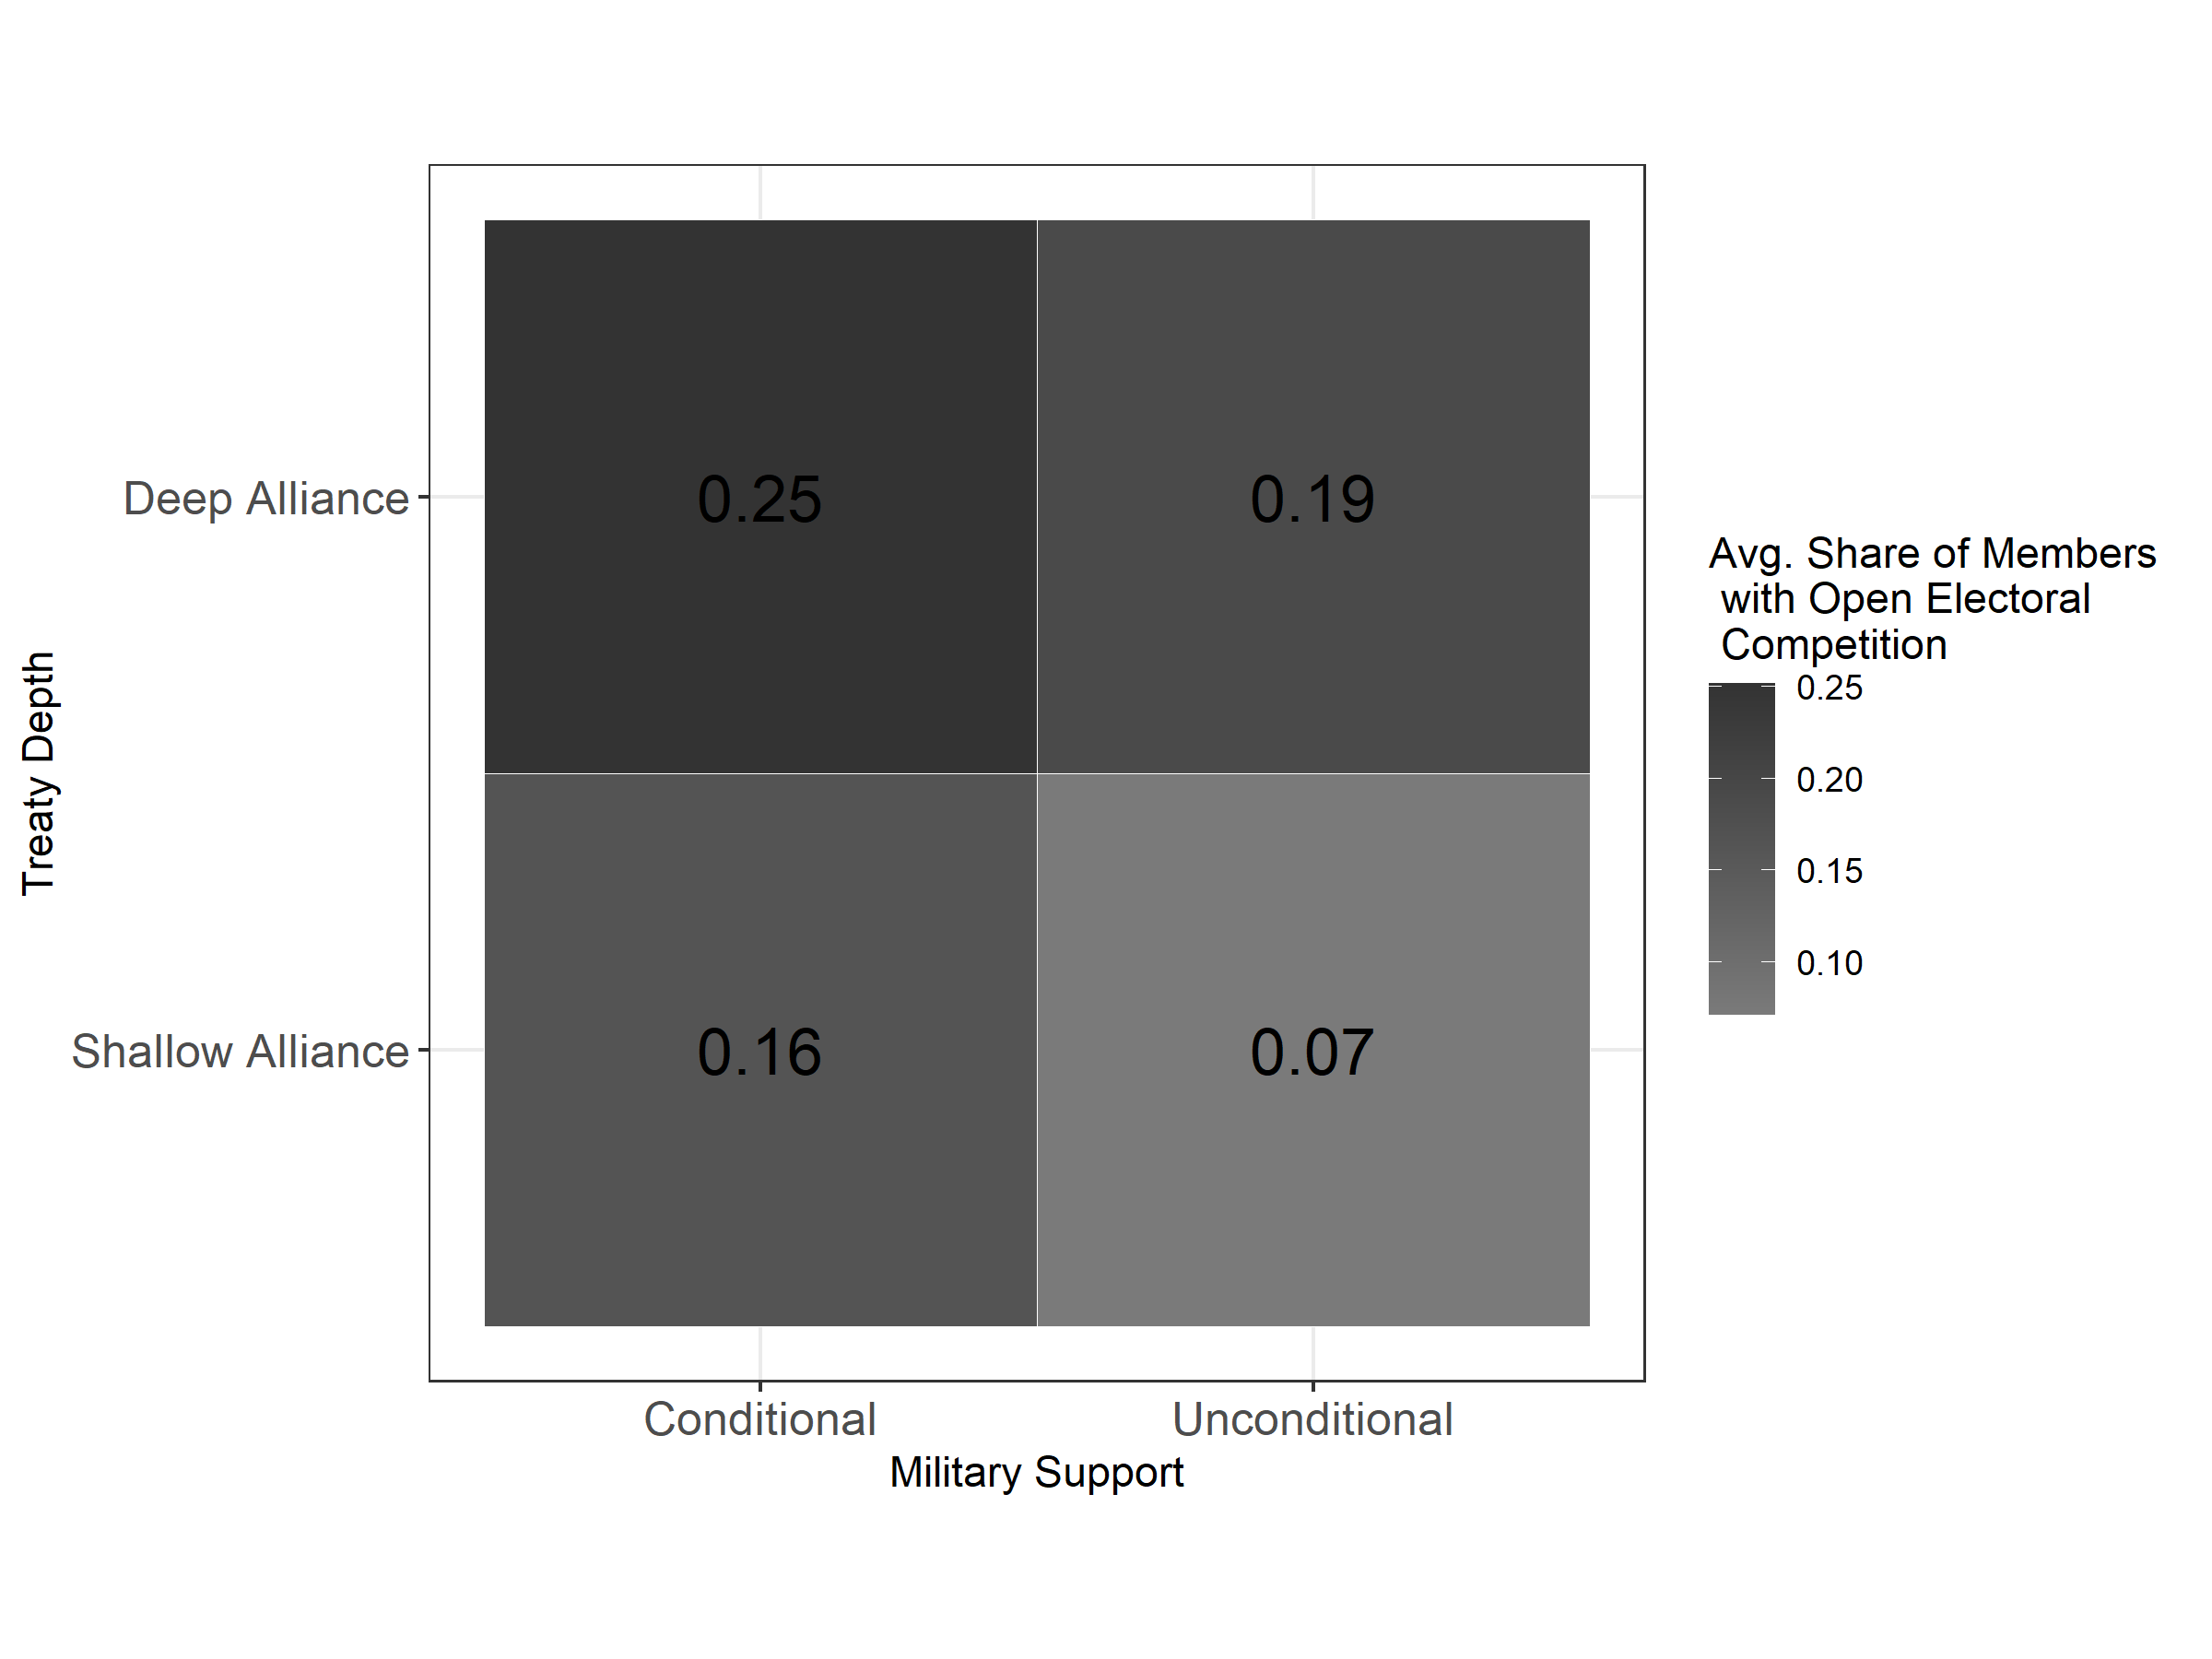
\includegraphics[width=.95\textwidth]{democ-prop-combo.png}  
\caption{Average proportion of democratic members in four groups of alliances. Alliances groups are based on treaty depth and unconditional military support.}
\label{fig:democ-prop-combo}
\end{figure}


In \autoref{tab:separate-models-prop}, I summarize the results from separate models of unconditional military support and treaty depth.
There is substantial uncertainty in the democratic proportion coefficient for both outcomes. 
These weaker than expected results may reflect differences in influence or the competing effects of democratic institutions I identified in the paper, or unmodeled error term correlations.\footnote{Inferences about unconditional military support may differ from \citet{Chibaetal2015} due to differences in the sample and model specifications.}



\begin{table}[!htbp] \centering 
  \caption{} 
  \label{tab:separate-models-prop} 
\begin{tabular}{@{\extracolsep{5pt}}lcc} 
\\[-1.8ex]\hline 
\hline \\[-1.8ex] 
 & \multicolumn{2}{c}{\textit{Dependent variable:}} \\ 
\cline{2-3} 
\\[-1.8ex] & Latent Depth (rescaled) & Unconditional Military Support \\ 
\\[-1.8ex] & \textit{beta} & \textit{probit} \\ 
\\[-1.8ex] & (1) & (2)\\ 
\hline \\[-1.8ex] 
 Proportion of Democracies & 0.125 & $-$0.516 \\ 
  & ($-$0.334, 0.583) & ($-$1.176, 0.145) \\ 
  Foreign Policy Concessions & $-$0.092 & 0.006 \\ 
  & ($-$0.246, 0.061) & ($-$0.214, 0.227) \\ 
  Number of Members & 0.024$^{}$ & $-$0.031 \\ 
  & ($-$0.002, 0.050) & ($-$0.077, 0.015) \\ 
  Wartime Alliance & $-$0.275 & $-$0.980$^{}$ \\ 
  & ($-$0.624, 0.074) & ($-$1.597, $-$0.363) \\ 
  Asymmetric Obligations & 0.283$^{}$ & 0.038 \\ 
  & ($-$0.053, 0.619) & ($-$0.456, 0.532) \\ 
  Asymmetric Capability & 0.346 & 0.600 \\ 
  & ($-$0.123, 0.815) & ($-$0.269, 1.468) \\ 
  Non-Major Only & 0.253 & 1.093$^{}$ \\ 
  & ($-$0.254, 0.760) & (0.209, 1.977) \\ 
  Average Threat & 1.101$^{}$ & 1.645$^{}$ \\ 
  & (0.238, 1.965) & (0.328, 2.961) \\ 
  Foreign Policy Disagreement & 0.117 & 0.384 \\ 
  & ($-$0.339, 0.573) & ($-$0.312, 1.079) \\ 
  Start Year & 0.004$^{}$ & 0.015$^{}$ \\ 
  & (0.001, 0.008) & (0.010, 0.021) \\ 
  Constant & $-$9.468$^{}$ & $-$31.466$^{}$ \\ 
  & ($-$16.269, $-$2.668) & ($-$42.952, $-$19.979) \\ 
 \hline \\[-1.8ex] 
Observations & 277 & 277 \\ 
Log Likelihood & 52.250 & $-$132.053 \\ 
\hline 
\hline \\[-1.8ex] 
\textit{Note:}  & \multicolumn{2}{r}{95\% Confidence Intervals in Parentheses.} \\ 
\end{tabular} 
\end{table} 



Inferences about the proportion of democracies and alliance treaty design are sensitive to correlated errors in the depth and unconditional military support models, however. 
Results from a generalized joint regression model of treaty depth and unconditional military support match the findings in the paper, as \autoref{fig:results-prop} shows. 
There is a no substantive association between the proportion of democracies in an alliance and the probability of unconditional military support. 
Alliances between democracies have higher treaty depth, however. 
In this bivariate model alliance with more democracies are not more likely undertake conditional obligations, but there is a positive relationship between democratic alliance membership and treaty depth. 


\begin{figure}
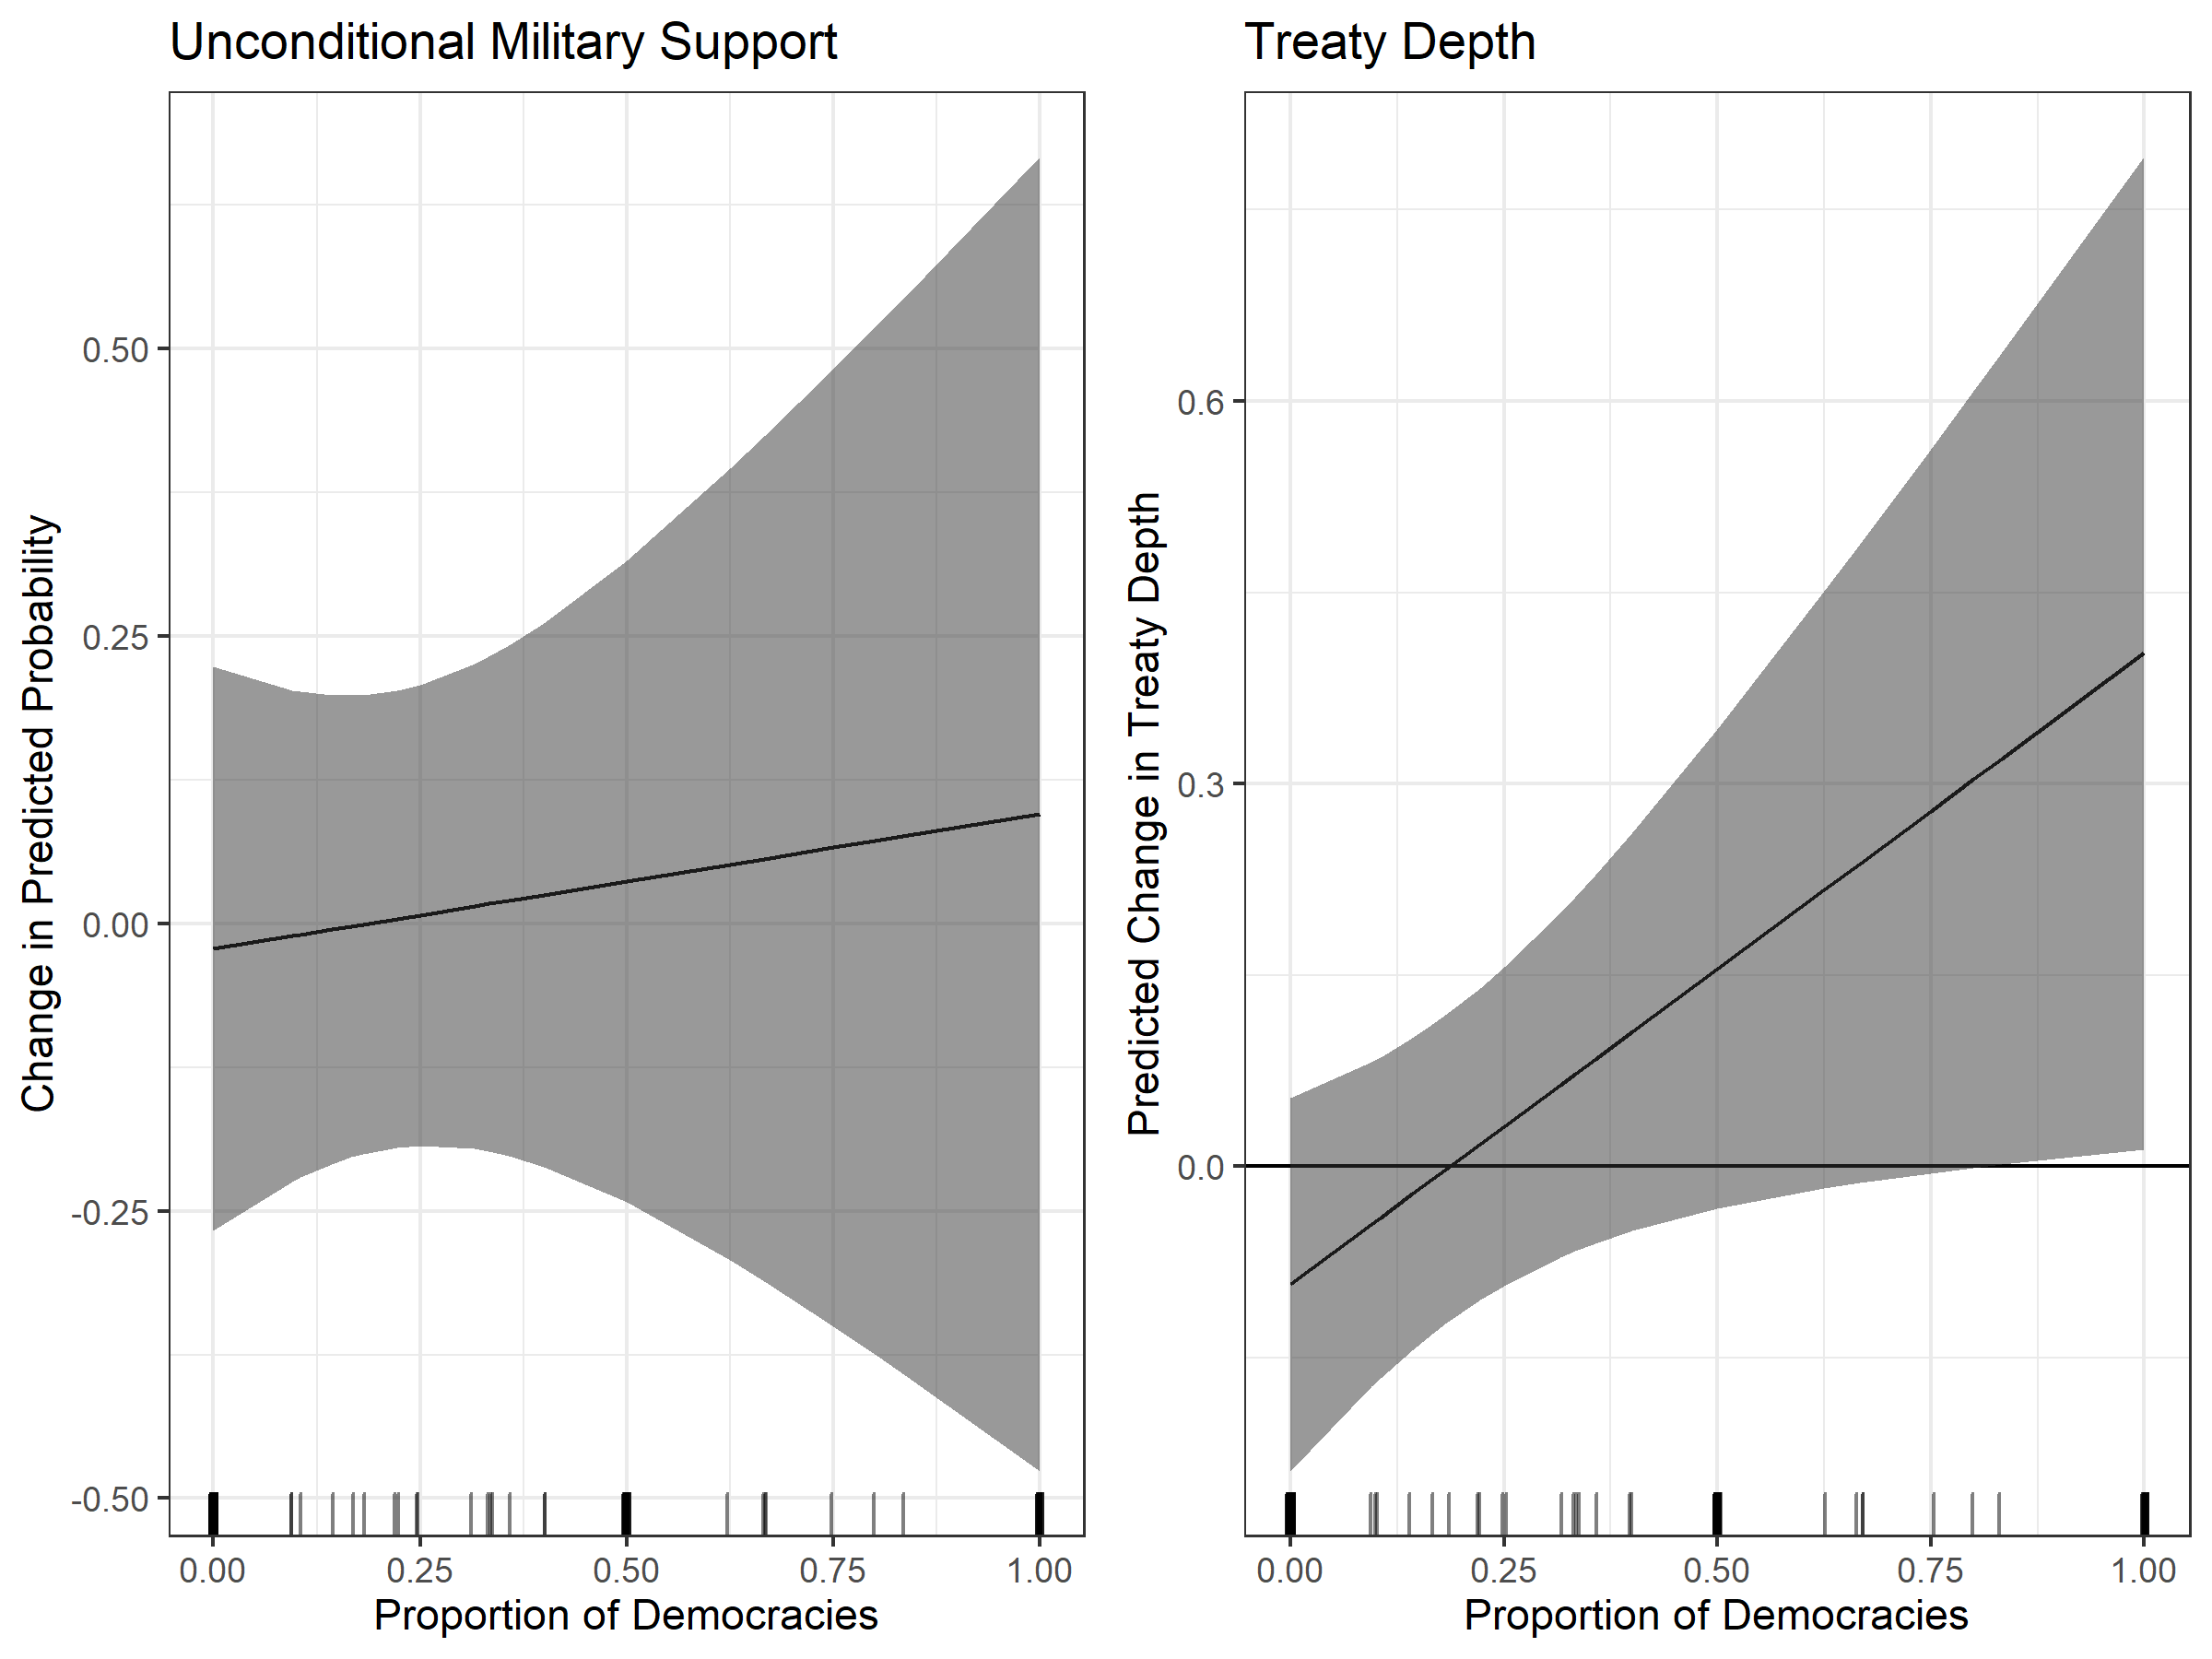
\includegraphics[width=.95\textwidth]{results-prop.png}  
\caption{Predicted change in probability of unconditional military support and predicted changes in treaty depth by the the proportion of democratic alliance members. The line marks predicted values, and the shaded areas encapsulate the standard errors. The rug plot on the x-axis marks observed values of allied democracy. Predictions based on the smoothed terms from the joint generalized regression model.}
\label{fig:results-prop}
\end{figure}


\section{Other Measures of Treaty Depth}


To address a highly skewed distribution and facilitate inferences across a wide range of estimation strategies, results in the paper are based on rescaled mean latent treaty depth, which ranges between 0 and 1. 
I modeled the rescaled outcome with a beta distribution. 
I make similar inferences about treaty depth and the Polity score of the most capable alliance member when I estimate regression models of treaty depth without this transformation, however. 
\autoref{tab:depth-alt-models} summarizes these results. 

\begin{table}[!htbp] 
\centering 
\begin{adjustbox}{width= .95\textwidth, center}
\begin{tabular}{@{\extracolsep{5pt}}lcccc} 
\\[-1.8ex]\hline 
\hline \\[-1.8ex] 
 & \multicolumn{4}{c}{\textit{Dependent variable:}} \\ 
\cline{2-5} 
\\[-1.8ex] & \multicolumn{3}{c}{Latent Depth} & Deep Alliance Dummy \\ 
\\[-1.8ex] & \textit{OLS} & \multicolumn{2}{c}{\textit{Robust Reg.}} & \textit{Probit} \\ 
\\[-1.8ex] & (1) & (2) & (3) & (4)\\ 
\hline \\[-1.8ex] 
 Alliance Leader Polity & 0.020$^{}$ & 0.019$^{}$ & 0.028$^{}$ & 0.030$^{}$ \\ 
  & (0.004, 0.035) & (0.003, 0.035) & (0.010, 0.046) & (0.004, 0.056) \\ 
  Foreign Policy Concessions & $-$0.043 & $-$0.043 & $-$0.104 & 0.006 \\ 
  & ($-$0.157, 0.070) & ($-$0.159, 0.073) & ($-$0.239, 0.030) & ($-$0.188, 0.199) \\ 
  Number of Members & 0.015 & 0.017 & 0.017 & 0.033$^{}$ \\ 
  & ($-$0.005, 0.036) & ($-$0.003, 0.038) & ($-$0.004, 0.037) & ($-$0.005, 0.071) \\ 
  Wartime Alliance & $-$0.253$^{}$ & $-$0.240$^{}$ & 0.040 & $-$0.429$^{}$ \\ 
  & ($-$0.511, 0.005) & ($-$0.505, 0.024) & ($-$0.306, 0.386) & ($-$0.877, 0.019) \\ 
  Asymmetric Obligations & 0.101 & 0.126 & 0.293$^{}$ & 0.339 \\ 
  & ($-$0.155, 0.356) & ($-$0.136, 0.388) & ($-$0.040, 0.625) & ($-$0.089, 0.767) \\ 
  Asymmetric Capability & 0.302$^{}$ & 0.283 & 0.212 & 0.671$^{}$ \\ 
  & ($-$0.043, 0.646) & ($-$0.070, 0.636) & ($-$0.499, 0.924) & (0.069, 1.273) \\ 
  Non-Major Only & 0.229 & 0.230 & 0.072 & 0.675$^{}$ \\ 
  & ($-$0.143, 0.601) & ($-$0.151, 0.611) & ($-$0.639, 0.783) & (0.029, 1.321) \\ 
  Average Threat & 0.963$^{}$ & 0.965$^{}$ & 1.424$^{}$ & 1.881$^{}$ \\ 
  & (0.317, 1.608) & (0.303, 1.626) & (0.650, 2.198) & (0.748, 3.014) \\ 
  Foreign Policy Disagreement & 0.180 & 0.161 & 0.333 & 0.279 \\ 
  & ($-$0.158, 0.517) & ($-$0.185, 0.507) & ($-$0.104, 0.770) & ($-$0.294, 0.853) \\ 
  Start Year & 0.003$^{}$ & 0.003$^{}$ & 0.021$^{}$ & 0.001 \\ 
  & (0.0003, 0.005) & (0.00001, 0.005) & (0.014, 0.027) & ($-$0.003, 0.006) \\ 
  Constant & $-$6.226$^{}$ & $-$5.789$^{}$ & $-$41.431$^{}$ & $-$4.431 \\ 
  & ($-$11.203, $-$1.249) & ($-$10.890, $-$0.688) & ($-$53.699, $-$29.162) & ($-$12.869, 4.006) \\ 
 \hline \\[-1.8ex] 
Observations & 279 & 279 & 203 & 279 \\ 
\hline 
\hline \\[-1.8ex] 
\textit{Note:}  & \multicolumn{4}{r}{95\% Confidence Intervals in Parentheses.} \\ 
\end{tabular}
\end{adjustbox} 
  \caption{Regression models of untransformed alliance treaty depth. Model 1 uses an OLS estimator, while Models 2 and 3 are robust regressions with Tukey's Biweight function. Model 3 includes data from 1919 to 2010. Model 4 is a binomial model of whether an alliance has median treaty depth or higher. All four models find a positive association between the Polity score of the most capable alliance member and treaty depth.} 
  \label{tab:depth-alt-models} 
\end{table} 


In \autoref{tab:depth-alt-models}, I include inferences from OLS, a robust regression estimator, and a probit GLM. 
The robust regression re-weights observations to correct for non-normal residuals and influential observations that might bias inferences from the OLS estimator. 
Model 3 is a robust regression of alliances after 1919, which is the time frame in \citet{Mattes2012}. 
In the probit model, the outcome is dummy variable that I set equal to one if the alliance has higher than the median latent depth. 


In addition to examining the association between democracy and depth without rescaling the outcome, I examine the association between alliance leader democracy and two measures from earlier scholarship that capture parts of treaty depth. 
First, \citet{LeedsAnac2005} develop an ordinal measure of military institutionalization.
Second, \citet{BensonClinton2016} use a latent variable model to measure treaty depth, but their concept views depth as the overall costliness of the alliance obligations. 
Although these two measures have limitations that make my measure a better fit for this paper, I find that the Polity score of the alliance leader is positively correlated with both variables.


Alliance leader democracy is positively correlated with the Leeds and Anac measure of military institutionalization in separate and joint models.
The ordinal military institutionalization measure is a useful first step towards measuring defense cooperation, but it understates the amount of variation in treaty depth. 
\citet{LeedsAnac2005} argue that commitments of an integrated military command, common defense policy, or any basing rights generate high military institutionalization. 
Official contact between military officials, formal organizations, providing training or technology, subordination of forces, or specific contributions reflect moderate institutionalization. 
If at least one of the relevant factors is present, Leeds and Anac assign the alliance the highest corresponding level of institutionalization. 
So an alliance with basing rights and subordination of forces has high institutionalization, but is just as institutionalized as an alliance with only basing rights, for example. 
This approach assumes that alliances with multiple sources of depth as just as deep/institutionalized as alliances with one source and understates the amount of variation in alliance treaty depth.


\begin{figure}[htbp]
	\centering
		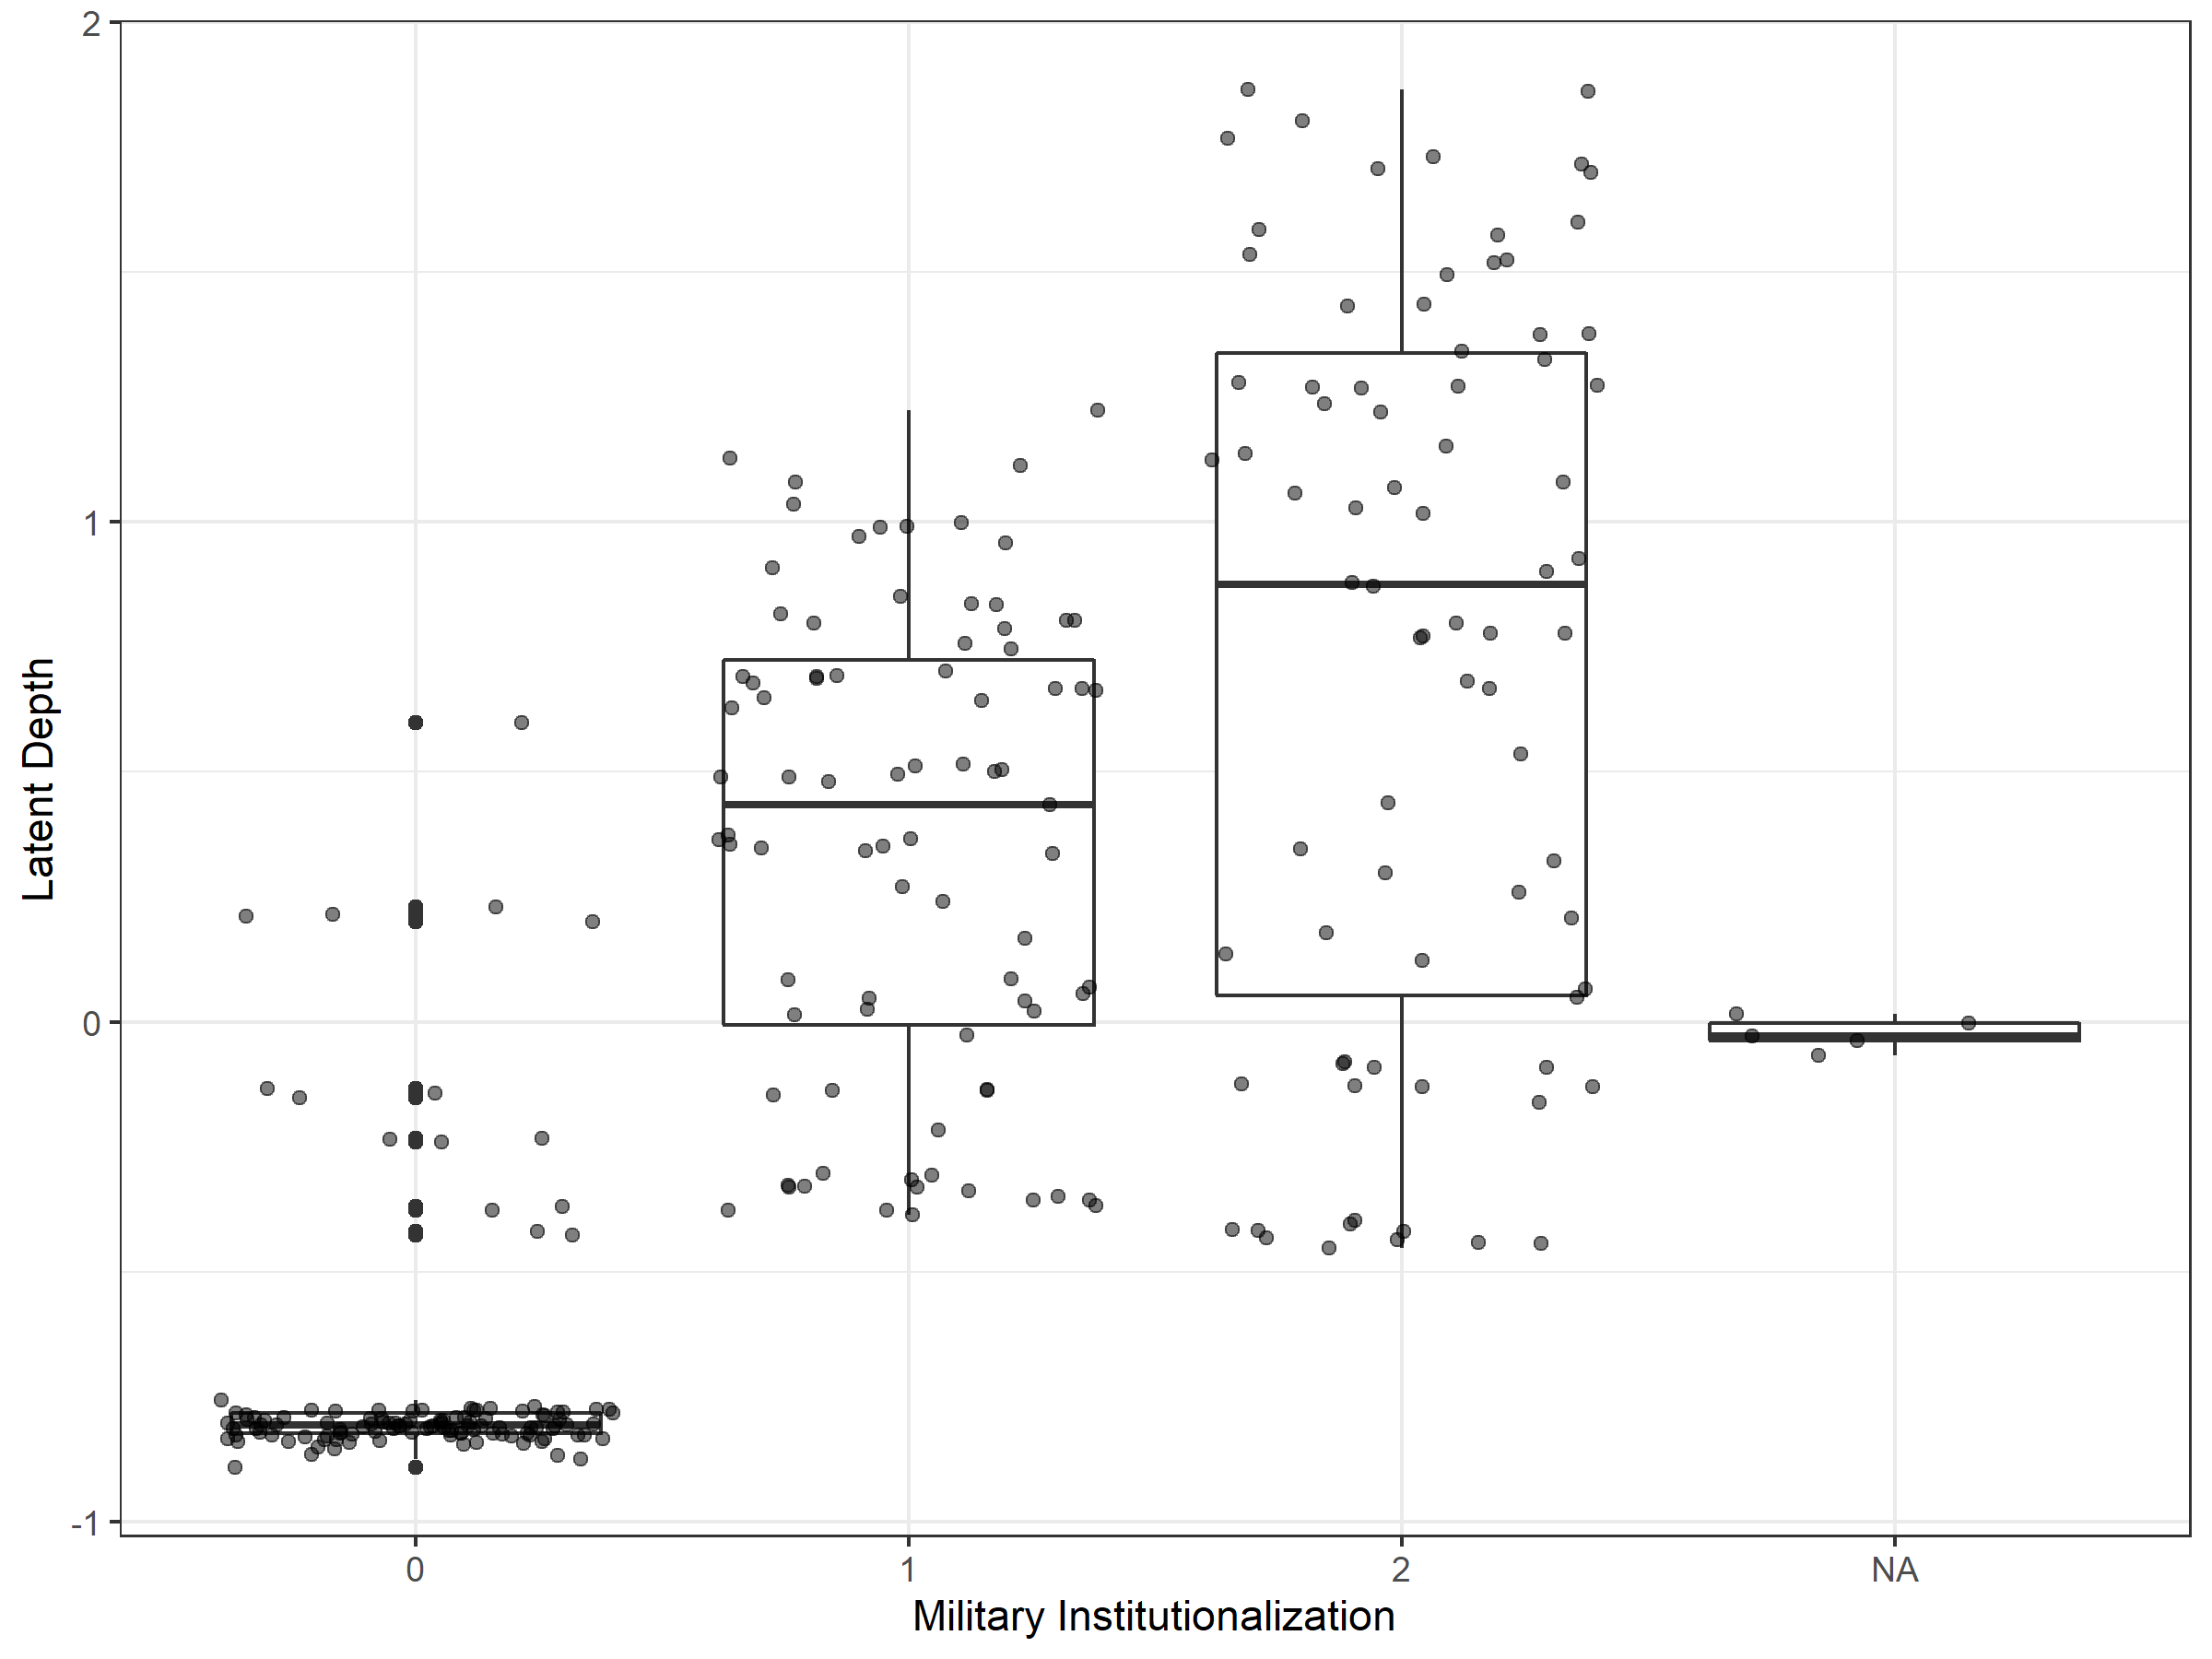
\includegraphics[width=0.95\textwidth]{milinst-comp.png}
	\caption{Scatter plot of latent treaty depth across the values of military institutionalization from \citet{LeedsAnac2005}. The box plots summarize the distribution of latent treaty depth within each category of military institutionalization. Points are jittered within each level of the institutionalization score.}
	\label{fig:milinst-comp}
\end{figure} 


As \autoref{fig:milinst-comp} shows, the ordinal variable is positively correlated with my latent measure, but there is substantial variation in latent depth within each level. 
The deepest alliances on the latent measure also have the highest military institutionalization score.
There are substantial differences within each category and overlap in the latent scores across the categories, however. 
For example, some alliances that \citet{LeedsAnac2005} assign a moderate institutionalization score have more depth than alliances with high institutionalization scores because these alliance treaties contain multiple sources of depth. 


\citet{BensonClinton2016}'s measure addresses a different concept, covers fewer alliances and their measurement model produces more outliers that may impact inferences.
Benson and Clinton's emphasis on the general costliness of the alliance means they include measures of issue linkages and secrecy, which are distinct from defense cooperation. 
Their measure is also based on version 3 of the ATOP data, so it has more limited temporal coverage. 
Last, their latent variable model makes a series of distributional assumptions that affect the estimated distribution of the latent variable. 
My latent variable model uses a semiparametric approach that accounts for dependencies between the factors and latent variables, so the distribution of the latent variable may be more accurate \citep{Murrayetal2013}.
For these three reasons, my latent measure better captures the concept of defense coordination and cooperation.\footnote{When scholars want to measure the overall costliness of alliance obligations, they should consider Benson and Clinton's measure.} 
Despite these differences, I find a positive association between the Polity score of the most capable alliance member and Benson and Clinton's measure of depth. 


I now discuss the results of analyses with both alternative dependent variables. 
As in the paper, I start with univariate models then estimate a bivariate model with each depth measure and unconditional military support. 
First, I fit an ordinal model of military institutionalization. 
Then, after rescaling Benson and Clinton's depth measure to range between 0 and 1, I fit a beta regression model. 
\autoref{fig:results-alt-measures-sep} plots the substantive effect of the most capable alliance member's Polity score on both outcomes. 
Democratic institutions in the alliance leader increase the probability of high institutionalization and decrease the probability of no institutionalization. 
Alliance leader democracy is also positively associated with Benson and Clinton's measure of depth. 


\begin{figure}
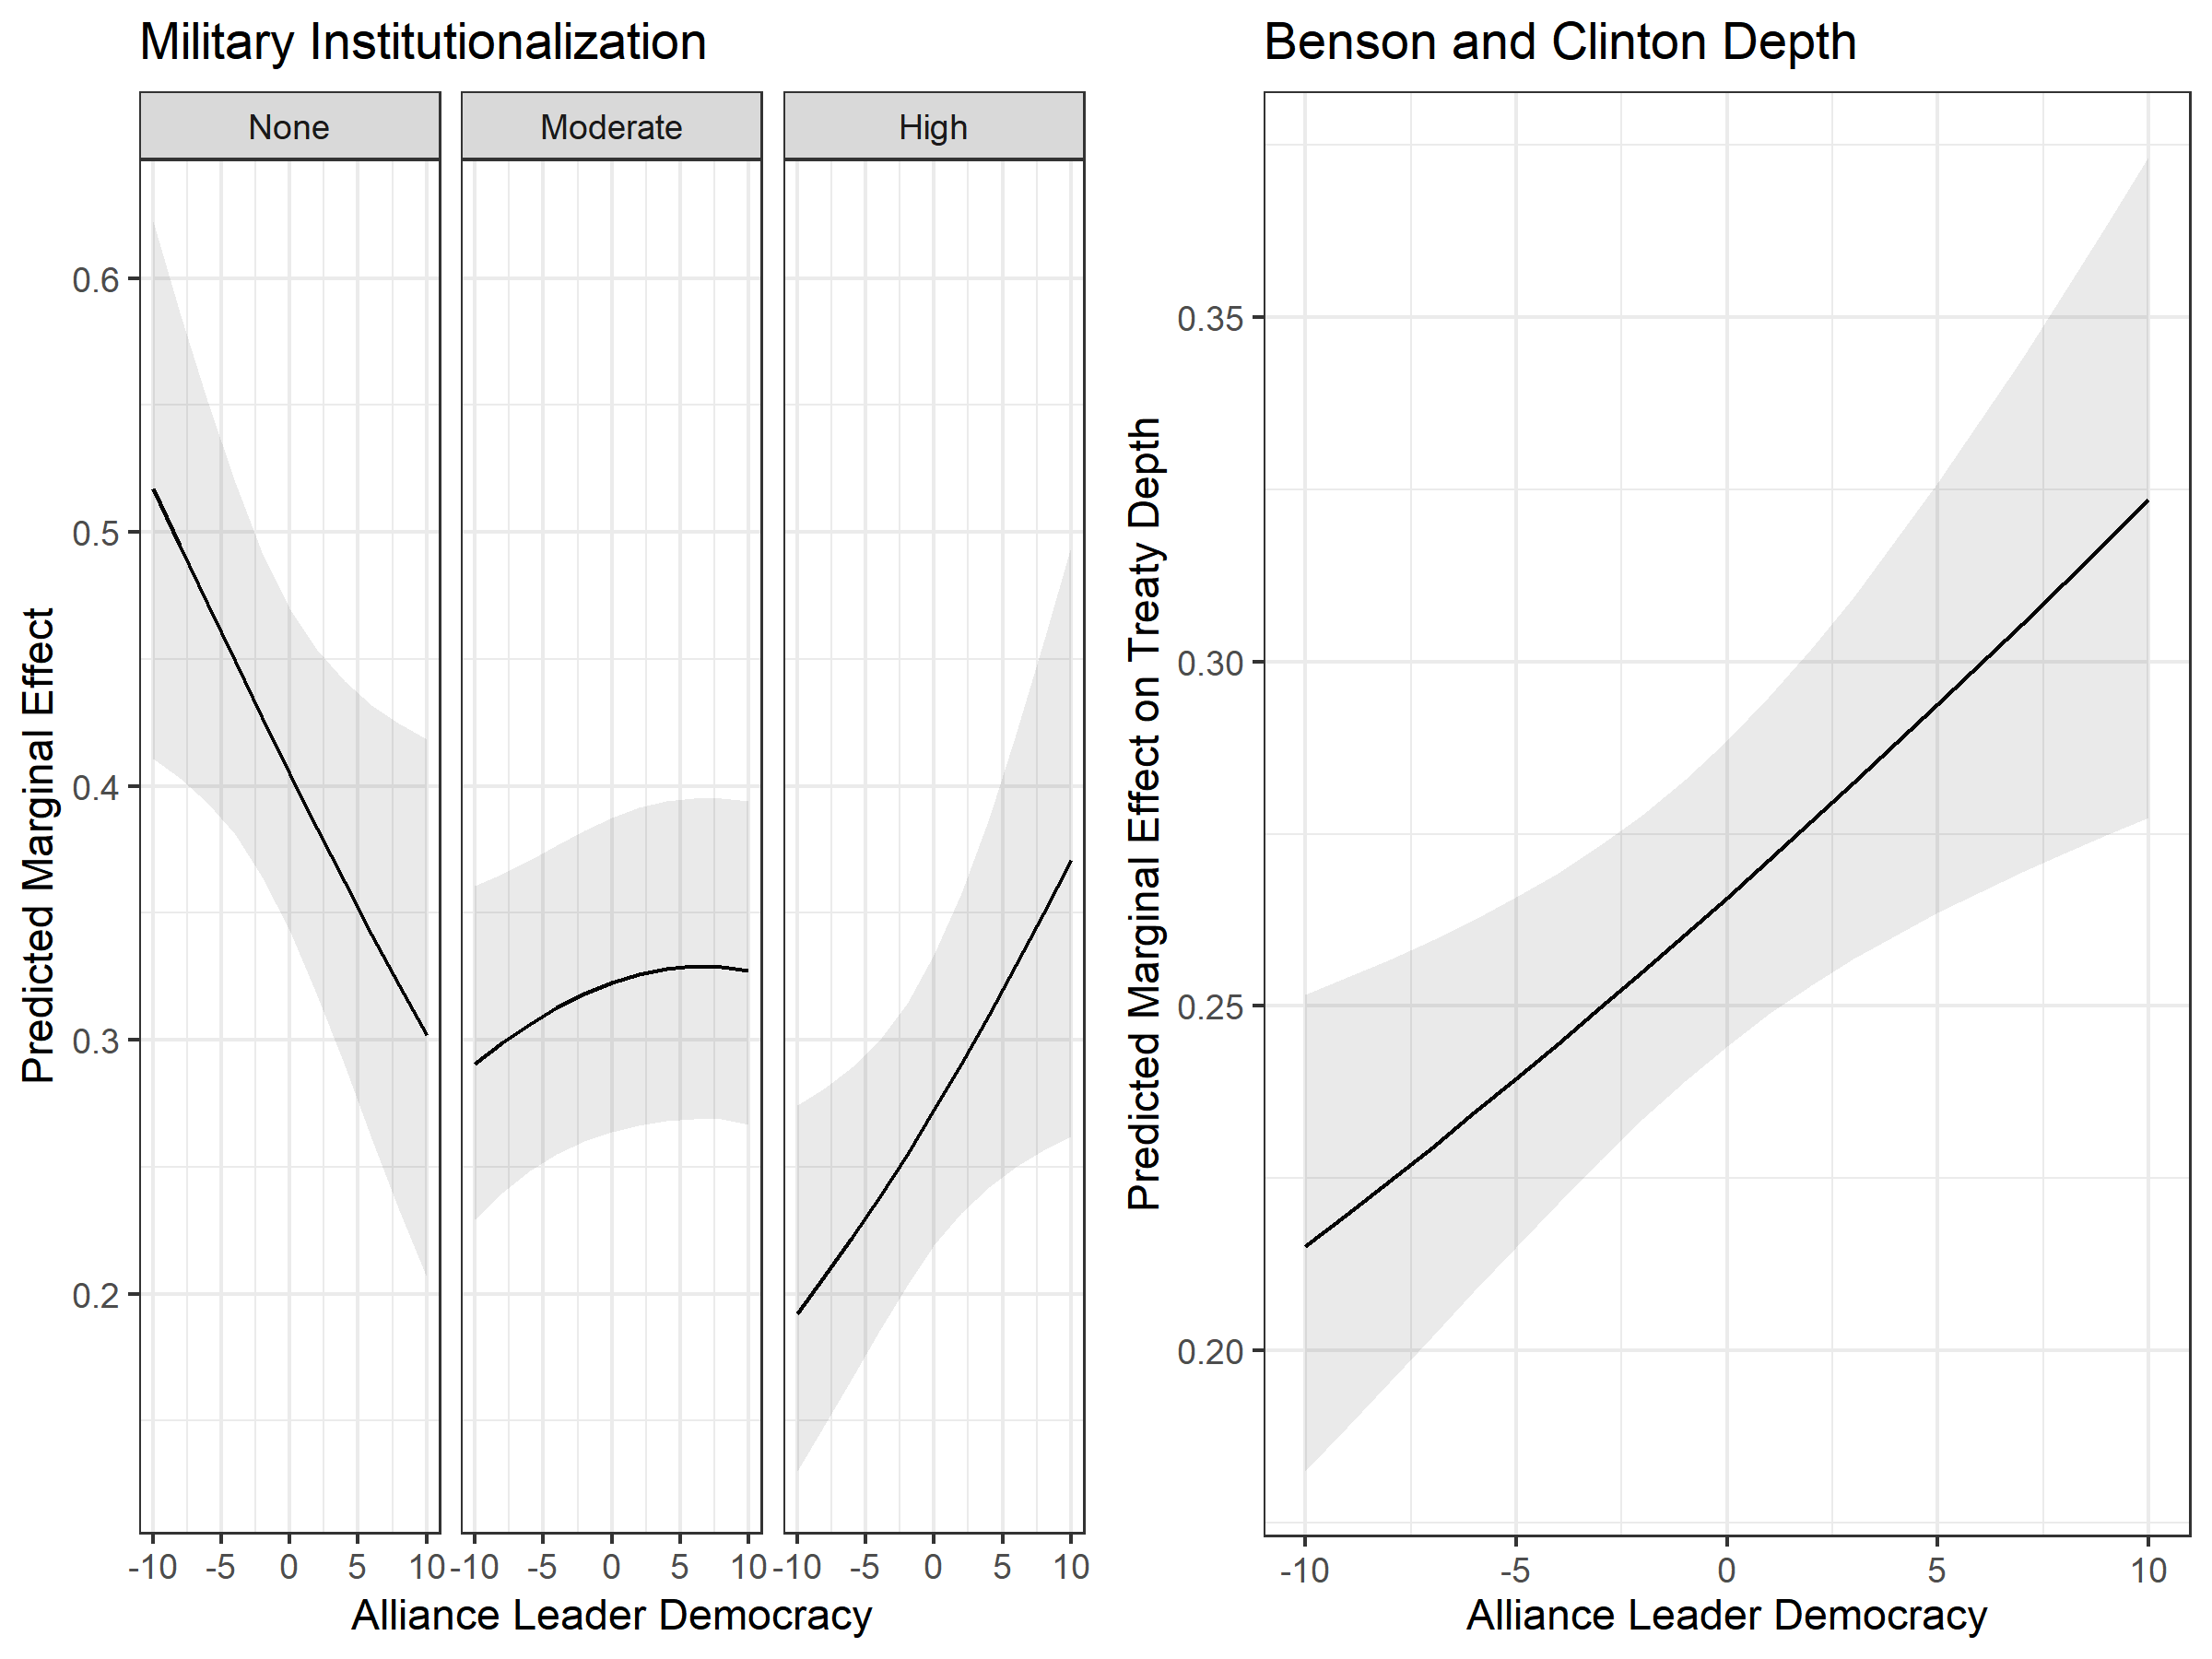
\includegraphics[width=.95\textwidth]{results-alt-measures-sep.png}  
\caption{Predicted changes in treaty depth by the Polity score of the most capable alliance member. The line marks predicted values, and the shaded areas encapsulate the 95\% confidence interval.}
\label{fig:results-alt-measures-sep}
\end{figure}


\autoref{fig:results-alt-measures} plots predictions from the two alternative depth measures based on bivariate models. 
For the military institutionalization measure, I could not fit an ordinal model in GJRM.
Therefore, I created a dummy variable and set it equal to one if the alliance had high institutionalization. 
I then used a probit estimator to model the high military institutionalization dummy. 
The results of this analysis are weaker than expected. 
As the left panel of \autoref{fig:results-alt-measures} shows, although the the probability of high military institutionalization increases with alliance leader democracy, the increase is small. 
This may reflect limited variation in the ordinal measure, which I further reduced by translating it into a dummy variable. 


\begin{figure}
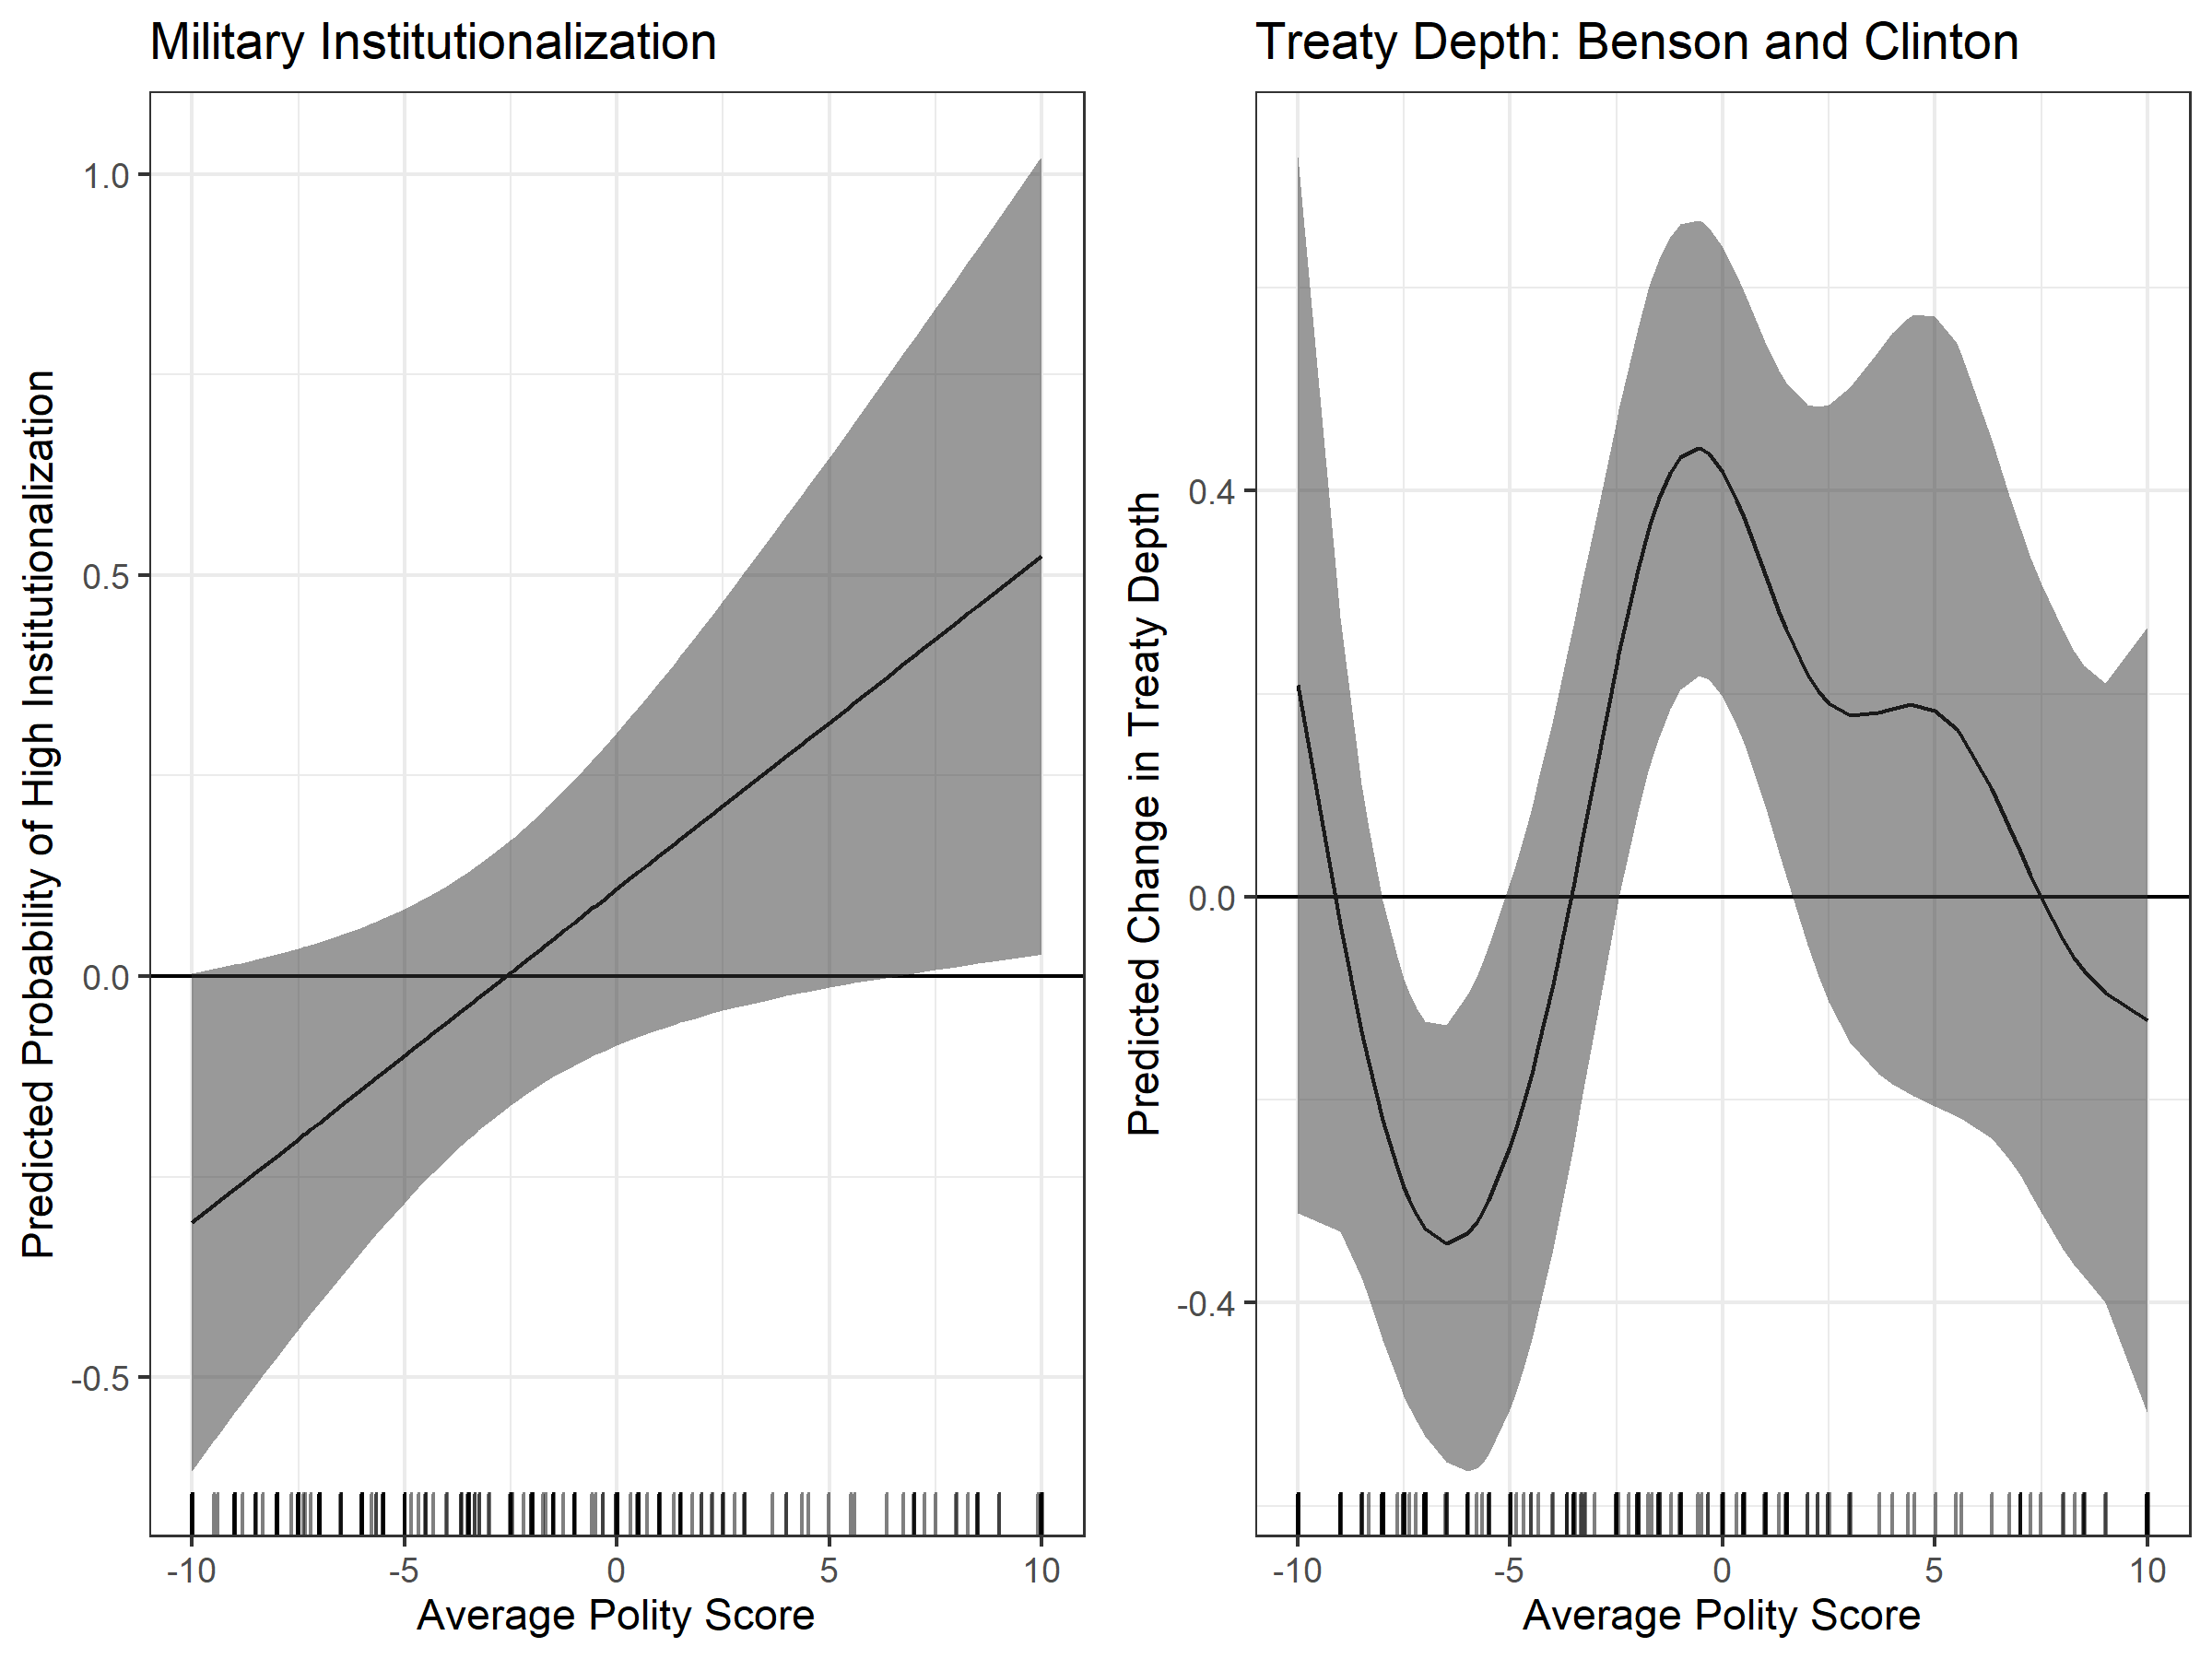
\includegraphics[width=.95\textwidth]{results-alt-measures.png}  
\caption{Predicted probability of military institutionalization and predicted treaty depth as a function of alliance leader democracy. The line marks predicted values, and the error bars summarize the approximate 95\% confidence interval. Predictions based on the smoothed terms from two joint generalized regression models, one for high military institutionalization and unconditional support, and another with Benson and Clinton's depth measure and unconditional military support. }
\label{fig:results-alt-measures}
\end{figure}


Findings about the association between treaty depth and Benson and Clinton's also match the treaty depth hypothesis. 
Moving from an autocratic to a democratic alliance leader increases the overall costliness of the alliance obligations. 
I suspect that this result is driven by the defense cooperation measures in Benson and Clinton's latent variable. 
In summary, I find similar results with four alternative measures of treaty depth, including two measures from previous scholarship. 




\section{Are Deep Alliances Less Reliable?} 


\citet{LeedsAnac2005} find that institutionalized alliances are less reliable, which contradicts my claim that deep alliances increase treaty reliability. 
Besides potential bias from non-random selection into challenges of alliances \citep{Smith1995}, this empirical finding depends in part on their ordinal measure. 
Replacing the ordinal institutionalization measure with my latent depth variable leads to difference inferences about alliance treaty design and performance. 
Therefore, the surprising finding in this paper that better institutionalized alliances have worse performance may also reflect measurement decisions. 


I focus my replication on Leeds and Anac's model of whether alliance members honor treaties with active military support. 
The replication focuses on this model because my argument examines defensive and offensive alliances. 
Their dataset includes 103 alliance performance opportunities, where states could honor or violate promises of military support. 
Using a logit model that adjusts for alliance formality, capability changes, changes in the policy process and whether the ally was the original target, Leeds and Anac find a negative relationship between institutionalization and performance. 
I replicate this estimate in the first column of \autoref{tab:depth-performance}. 


\begin{table}[!htbp] \centering 
  \caption{} 
  \label{tab:depth-performance} 
\begin{adjustbox}{width= .95\textwidth, center}
\begin{tabular}{@{\extracolsep{5pt}}lccc} 
\\[-1.8ex]\hline 
\hline \\[-1.8ex] 
 & \multicolumn{3}{c}{\textit{Dependent variable:}} \\ 
\cline{2-4} 
\\[-1.8ex] & \multicolumn{2}{c}{Leeds and Anac} & Berkemeier and Fuhrmann \\ 
\\[-1.8ex] & (1) & (2) & (3)\\ 
\hline \\[-1.8ex] 
 Military Institutionalization & $-$0.543 &  &  \\ 
  & ($-$1.306, 0.221) &  &  \\ 
  Latent Depth &  & 0.173 & 0.373 \\ 
  &  & ($-$0.583, 0.929) & ($-$0.384, 1.131) \\ 
  Alliance Formality & $-$1.161$^{}$ & $-$1.512$^{}$ &  \\ 
  & ($-$2.082, $-$0.240) & ($-$2.466, $-$0.558) &  \\ 
  Capability Change & $-$1.841$^{}$ & $-$1.928$^{}$ &  \\ 
  & ($-$3.135, $-$0.547) & ($-$3.251, $-$0.604) &  \\ 
  Process Change & $-$1.802$^{}$ & $-$1.462$^{}$ &  \\ 
  & ($-$3.336, $-$0.269) & ($-$2.886, $-$0.039) &  \\ 
  Original Target & $-$0.723 & $-$0.788 &  \\ 
  & ($-$1.849, 0.403) & ($-$1.942, 0.366) &  \\ 
  Asymmetric Capability &  &  & $-$2.832$^{}$ \\ 
  &  &  & ($-$5.230, $-$0.434) \\ 
  Non-Major Only &  &  & $-$2.036$^{}$ \\ 
  &  &  & ($-$4.286, 0.213) \\ 
  Post 1945 &  &  & $-$2.396$^{}$ \\ 
  &  &  & ($-$3.958, $-$0.834) \\ 
  Open Electoral Competition &  &  & 0.018 \\ 
  &  &  & ($-$1.003, 1.039) \\ 
  Executive Constraints &  &  & 1.420$^{}$ \\ 
  &  &  & ($-$0.254, 3.093) \\ 
  Number of Members &  &  & $-$0.233$^{}$ \\ 
  &  &  & ($-$0.487, 0.021) \\ 
  Economic Issue Linkage &  &  & $-$0.434 \\ 
  &  &  & ($-$1.573, 0.705) \\ 
  Unconditional Support &  &  & 1.047 \\ 
  &  &  & ($-$0.646, 2.739) \\ 
  Foreign Policy Concessions &  &  & $-$0.191 \\ 
  &  &  & ($-$0.900, 0.517) \\ 
  Constant & 3.430$^{}$ & 3.163$^{}$ & 2.949$^{}$ \\ 
  & (1.972, 4.888) & (1.766, 4.559) & (0.633, 5.264) \\ 
 \hline \\[-1.8ex] 
Observations & 93 & 93 & 108 \\ 
Log Likelihood & $-$39.131 & $-$40.039 & $-$48.046 \\ 
\hline 
\hline \\[-1.8ex] 
\textit{Note:}  & \multicolumn{3}{r}{95\% Confidence Intervals in Parentheses.} \\ 
\end{tabular}
\end{adjustbox} 
\end{table}


I then replace Leeds and Anac's institutionalization measure with my latent treaty depth measure, which is in the second column of \autoref{tab:depth-performance}. 
The coefficient on depth, in contrast to military institutionalization, is positive, though neither estimate is statistically significant at conventional levels. 
Thus, the possible direction of this association shifts, depending on how alliance depth is measured.


To further assess this finding, I utilized an updated alliance performance dataset from \citet{BerkemeierFuhrmann2018}.
In this case, I specified a different logit model that included latent depth, unconditional support, dummy indicators of asymmetric capability and symmetric non-major power pacts, a post 1945 dummy, the two indicators of democratic institutions, the number of members, economic issue linkages, and foreign policy concessions. 
All of these factors are potential sources of reliability, per different arguments in the literature. 
In these models, I find a similar result--- a positive relationship between depth and honoring military support that cannot be distinguished from zero.


In summary, I do not find that highly institutionalized alliances are less reliable. 
The change in the direction of the coefficient is more meaningful than a difference in statistical significance, given the limited number of alliance performance opportunities in these datasets. 
Again, given issues with non-random selection into alliance crises and challenges, one should not place too much weight on the above results. 
They do suggest, however, that deep alliances are not necessarily less reliable when invoked. 


\section{Adjusting for Alliance Formation}


Observed alliances are the result of negotiations between potential members. 
Therefore the set of observed alliances is not a random sample.
Rather, alliance members overcame the many obstacles to alliance formation \citep{Poast2019a}.  
In this section, I account for non-random alliance formation using a hurdle model of observed alliances after combining a stratified random sample of non-allied groups of states with observed alliances. 
This research design produces similar inferences: the Polity score of the most capable alliance member increases treaty depth but has no effect on unconditional military support. 


My research design for this robustness check follows established procedures for dealing with selection into alliances and treaty design. 
I followed the suggestions of \citet{Poast2010} for using k-adic data, because some alliances have more than two members. 
First I constructed a random sample of groups of states that could have formed an alliance in each year, but did not \citep{FordhamPoast2014}.
Then I took a stratified sample of the non-allied k-ads to include five times as many non-allied observations as alliance observations for each observed value of alliance size. 
For example, there are 215 bilateral alliances, so I sampled 1075 non-allied bilateral groups. 
There is only one alliance with 34 members, so I added five non-alled k-ads with 34 members. 
Finally, I summarized key characteristics of these non-allied k-ads, including average Polity score, the Polity score of the most capable member, the number of members, mean threat, asymmetric capability, and wartime, and merged the non-allied data with the observed alliance data. 


To model alliance treaty alliance design, I used the research design of \citet{Chibaetal2015}, who estimated a hurdle model to assess whether democracies were more likely to offer conditional obligations.
Hurdle models have two stages or parts, which can account for non-random selection into alliances.
A first stage model predicts which observations clear the hurdle to a second stage with non-zero outcome values. 
Observed alliances are the set of observations that cleared the hurdle and have an alliance treaty. 
Unlike a sample selection model, the second stage in a hurdle model is logically undefined, which is how alliance treaty design works.\footnote{Hurdle models also do not require an exclusion restriction for identification.} 
Unless states overcome the barriers to alliance formation, no agreed treaty content exists. 


Unlike \citet{Chibaetal2015}, however, I examine two aspects of alliance treaty design. 
Therefore, I estimate a bivariate hurdle model- one for the depth and the other for unconditional military support. 
To have zero values for the outcome at the hurdle stage, I adjusted the outcomes in these models. 
First, I shifted the scale of latent treaty depth by adding one, which shifted the distribution onto uniformly positive values. 
I then applied a gamma hurdle model to this rescaled depth outcome.  
For unconditional military support, I replaced the dummy variable in the manuscript with an ordinal indicator.
This ordinal variable captures the relative strength of the military support promise in the alliance. 
ATOP alliances can be conditional on four things: adversaries, locations, a particular conflict, the number of opponents, a specific demand or non-provocation in the case of defense treaties. 
The maximum number of observed conditions in an alliance is four, which is the most conditional and limited alliance in the data. 
I therefore invert the number of conditions and assign unconditional alliances a value of four. 
Essentially, the measure then captures the number of circumstances where an alliance could have applied conditions but did not. 
To avoid including zeros in observed alliances, because 0 is the value for groups with no alliance, I add one to the count of conditions.
Adding one also reflects how promising military support adds a base of commitment strength to any alliance \citep{Morrow2000}. 
Thus, the final measure of military support commitment strength ranges between 1 and 5 for observed alliances, but is zero for non-alliances. 


In both models, I use average democracy, mean threat, asymmetric capability, wartime, and year varying intercepts to predict whether the group of states clears the alliance formation hurdle.
In the second stage, I use the democracy of the most capable alliance member, the number of members, mean threat, dummy indicators of asymmetric capability or non-major power only membership, wartime and year varying intercepts to model treaty design. 
I then estimate the two hurdle models simultaneously using the BRMS package for \textsf{R}, which employs STAN for fully Bayesian inference \citep{Buerkner2017}. 
Unlike the GJRM estimators in the manuscripts, I cannot directly estimate residual correlations.
Instead, I connect the two hurdle models with a correlated set of year varying intercepts.\footnote{The complexity of this joint hurdle model and limited sample size in the second stage means results should be treated with caution. I find similar results with separate hurdle models for depth and conditions on military support. Results on file with the author.} 


Even after accounting for non-random alliance formation with the joint hurdle model, I find similar results to the manuscript. 
\autoref{fig:results-joint-hurdle} plots the results of the joint hurdle model. 
This figure shows the predicted marginal effect of alliance leader polity on commitment strength and shifted treaty depth, along with 90\% credible intervals.\footnote{Inferences from 90\% credible intervals in Bayesian models are more stable.} 
As in the sample with only observed alliances, greater democracy among alliance members increases treaty depth and has no clear relationship with conditions on military support. 


\begin{figure}
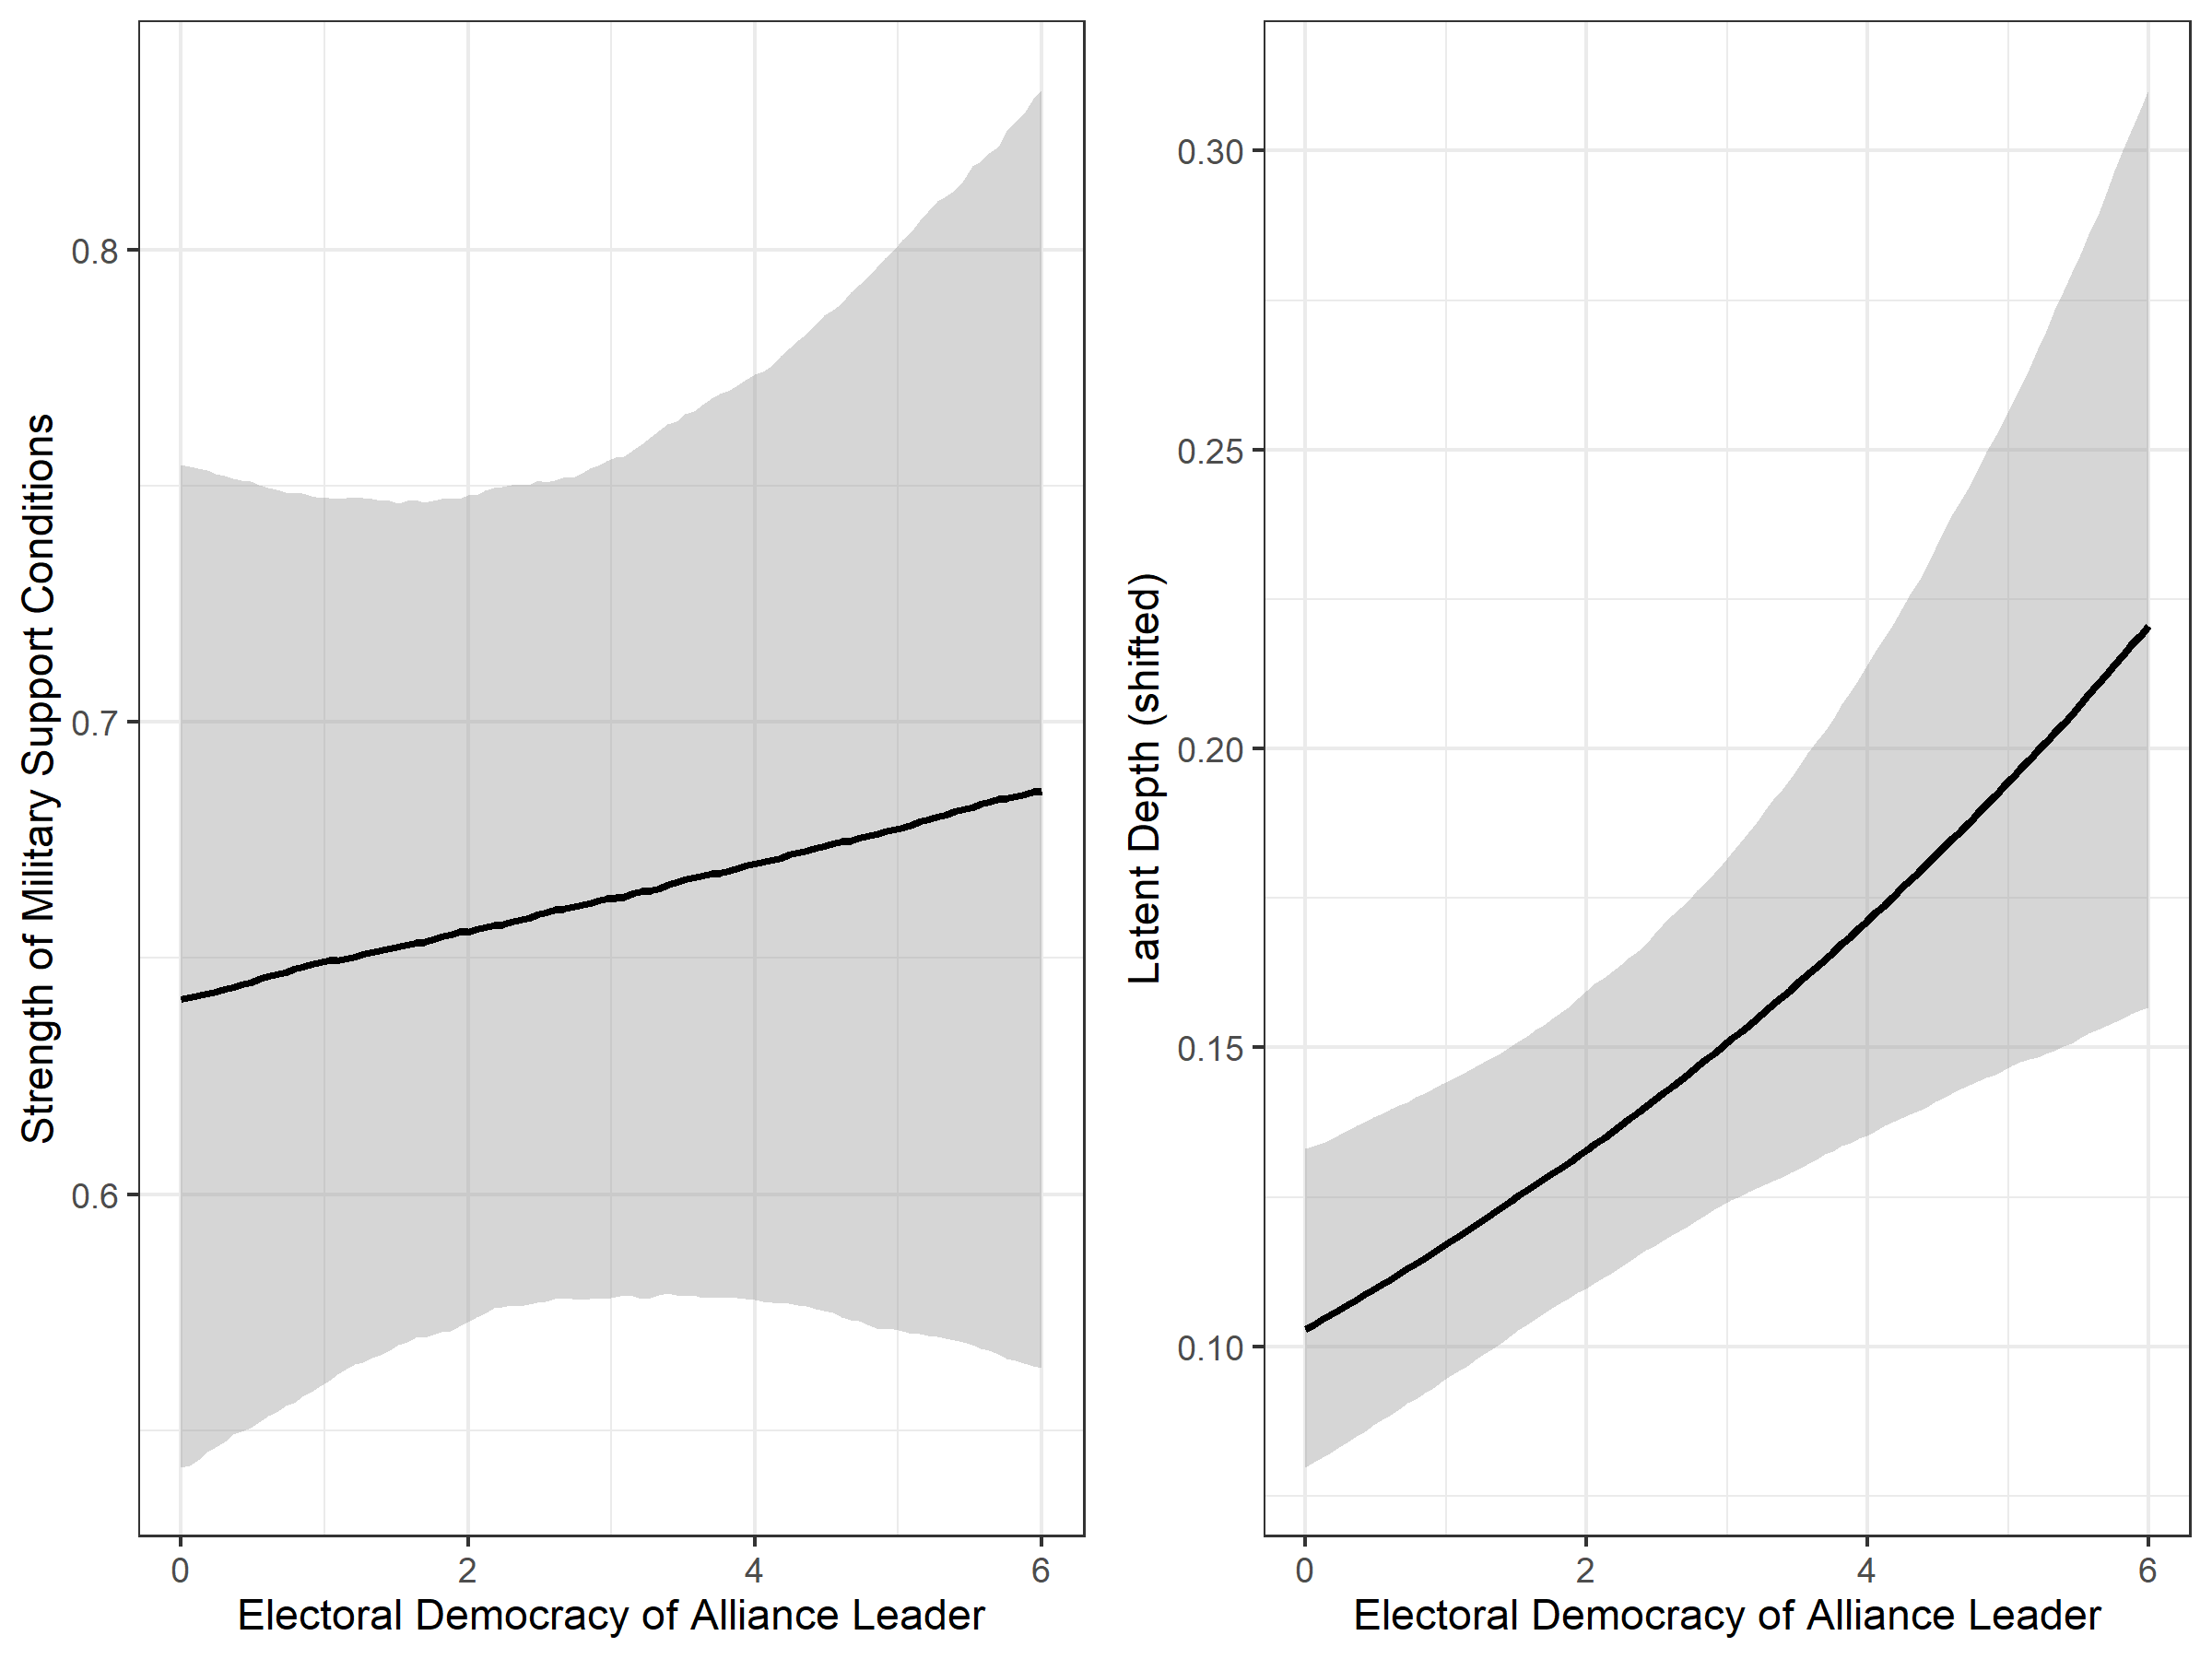
\includegraphics[width=.95\textwidth]{results-joint-hurdle.png}  
\caption{Predicted commitment strength and changes in treaty depth by the the average Polity score of alliance members when the treaty formed based on a joint hurdle model of alliances. The line marks predicted values, and the shaded areas encapsulate the 90\% credible interval. The rug plot on the x-axis marks observed values of allied democracy. Predictions hold all other variables constant.}
\label{fig:results-joint-hurdle}
\end{figure}




\section{Uncertainty in Latent Treaty Depth} 


In a further robustness check, I consider how measurement uncertainty shapes inferences about the connection between non-major power alliances and treaty depth. 
Although there are perceptible differences in treaty depth, especially once states add substantial depth to the treaty, the latent measure of treaty depth has some uncertainty. 
This uncertainty in the latent measure is common to all measurement models and offers a reasonable approximation of alliance politics, because the implications of alliance treaty design are uncertain.  


To incorporate uncertainty over treaty depth, I fit a modification of the joint model. 
First, I created 1,000 alliance datasets, one for each draw of the posterior distribution of the latent measure.
All other variables remained the same, but the treaty depth values are unique to each dataset. 
Then I fit the treaty depth model on 500 randomly sampled datasets from those 1,000 using Bayesian estimation through BRMS \citep{Buerkner2017}. 
Joint Bayesian estimation has the flexibility to incorporate the probit and beta models and can be easily extended to account for uncertainty in the depth measure, but it does not allow correlated errors. 
Fitting the model sequentially to each dataset produces 500 separate models, which I combine into a single model by aggregating the posterior draws into a unified posterior that accounts for uncertainty in the treaty depth measure.\footnote{Standard convergence diagnostics indicate convergence in all 500 models. Diagnostics like $\hat{r}$ are less useful for the full posterior, because some of the chains in the submodels do not overlap.}
This approach is analogous to common techniques for analyzing missing data, where multiple imputation generates uncertainty about the missing values \citep{Hollenbachetal2018imp}.
After multiple imputation, researchers fit a separate model to each imputed dataset and then combine the results. 


% Expand on these results later 
Even after accounting for uncertainty in the treaty depth measure, I find a similar pattern, albeit with more uncertainty in the estimates. 
I plot the relevant posterior distributions in \autoref{fig:results-unc-depth}. 
The 90\% credible interval for treaty depth barely overlaps zero, but 91\% of the posterior mass is positive. 
For unconditional military support, the 90\% credible interval has substantial uncertainty, but the alliance leader Polity has 88\% negative posterior probability. 
Thus the preponderance of evidence from these estimates matches the hypotheses. 


\begin{figure}
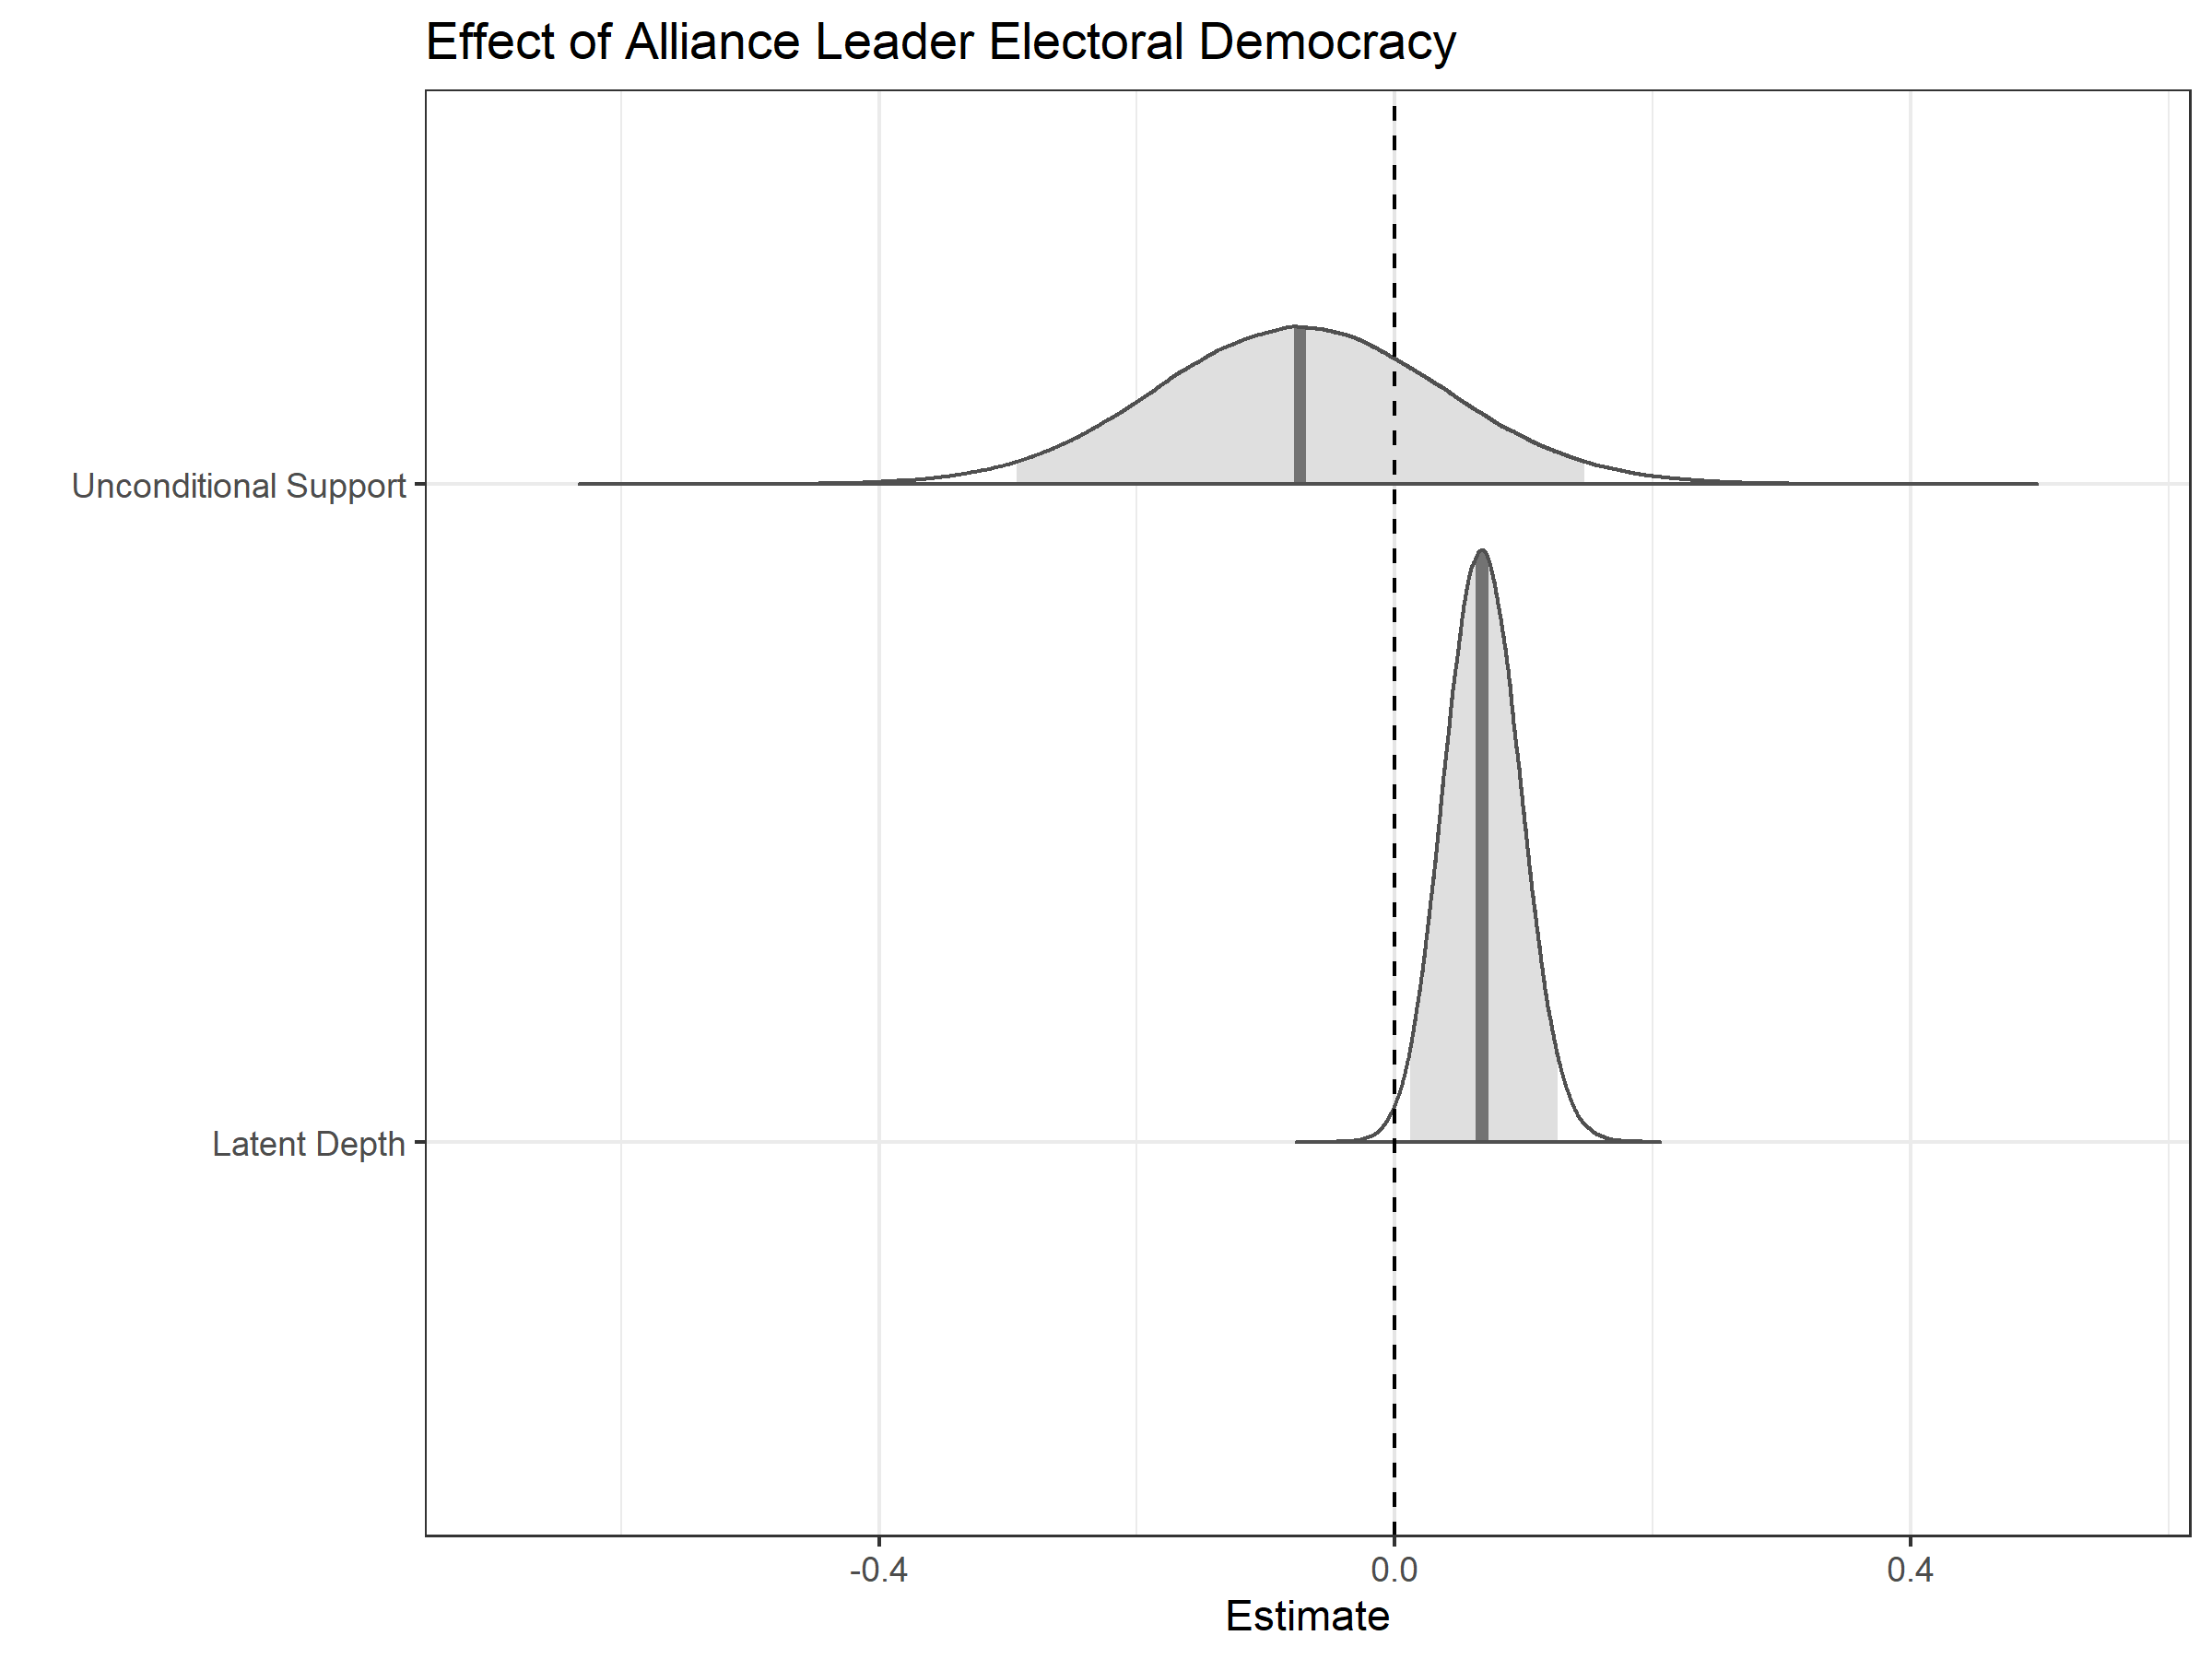
\includegraphics[width=.95\textwidth]{results-unc-depth.png}  
\caption{Estimated association between the democracy of the most capable alliance member and two sources of treaty depth from a Bayesian model that accounts for uncertainty in the latent depth measure. The density plot shows the posterior distributions, and the shaded area summarizes the 90\% credible interval.}
\label{fig:results-unc-depth}
\end{figure}



\section{Issue Linkages and Treaty Credibility}


\citep{Poast2013} observes that issue linkages increase alliance credibility in buffer states.
Buffer states face significant threats because they are located between competing major powers. which makes generating credible commitments difficult.
Because issue linkages make alliance commitments more credible in this ``hard case,'' Poast concludes that issue linkages are generally a source of credibility.
In the manuscript, I use issue linkages as a control variable and do not discuss them in the theory. 
I offer minimal discussion of issue linkages to simplify the argument and empirical tests. 
Examining treaty depth, unconditional military support and issue linkages together is a logical next step in theory development. 
For this paper, I also find a positive association between alliance leader democracy and treaty depth in a trivariate model of treaty depth, unconditional military support and issue linkages. 


The trivariate model uses three dummy variables to measure the outcomes, as this is a limitation of the GJRM estimator. 
The depth dummy is equal to one if an alliance has greater than the median value of latent treaty depth. 
Unconditional military support is equal to one if the alliance places no conditions on military intervention. 
Last, I set the issue linkages dummy equal to one if the alliance promises economic cooperation. 
The trivariate model converges to the same estimates regardless of the copula, so the results below should be interpreted with some caution.


Even after accounting for correlated errors between models of treaty depth, unconditional military support and issue linkages, I find a positive relationship between the Polity score of the most capable alliance member and treaty depth. 
I also find no clear association between the political institutions of the alliance leader and the probability of unconditional military support. 
\autoref{fig:pred-trivar} summarizes the predicted probabilities of each credibility source for the values of the alliance leaders' Polity score. 
Estimates hold all variables besides the Polity score of the most capable alliance member at their mode or median.  


\begin{figure}
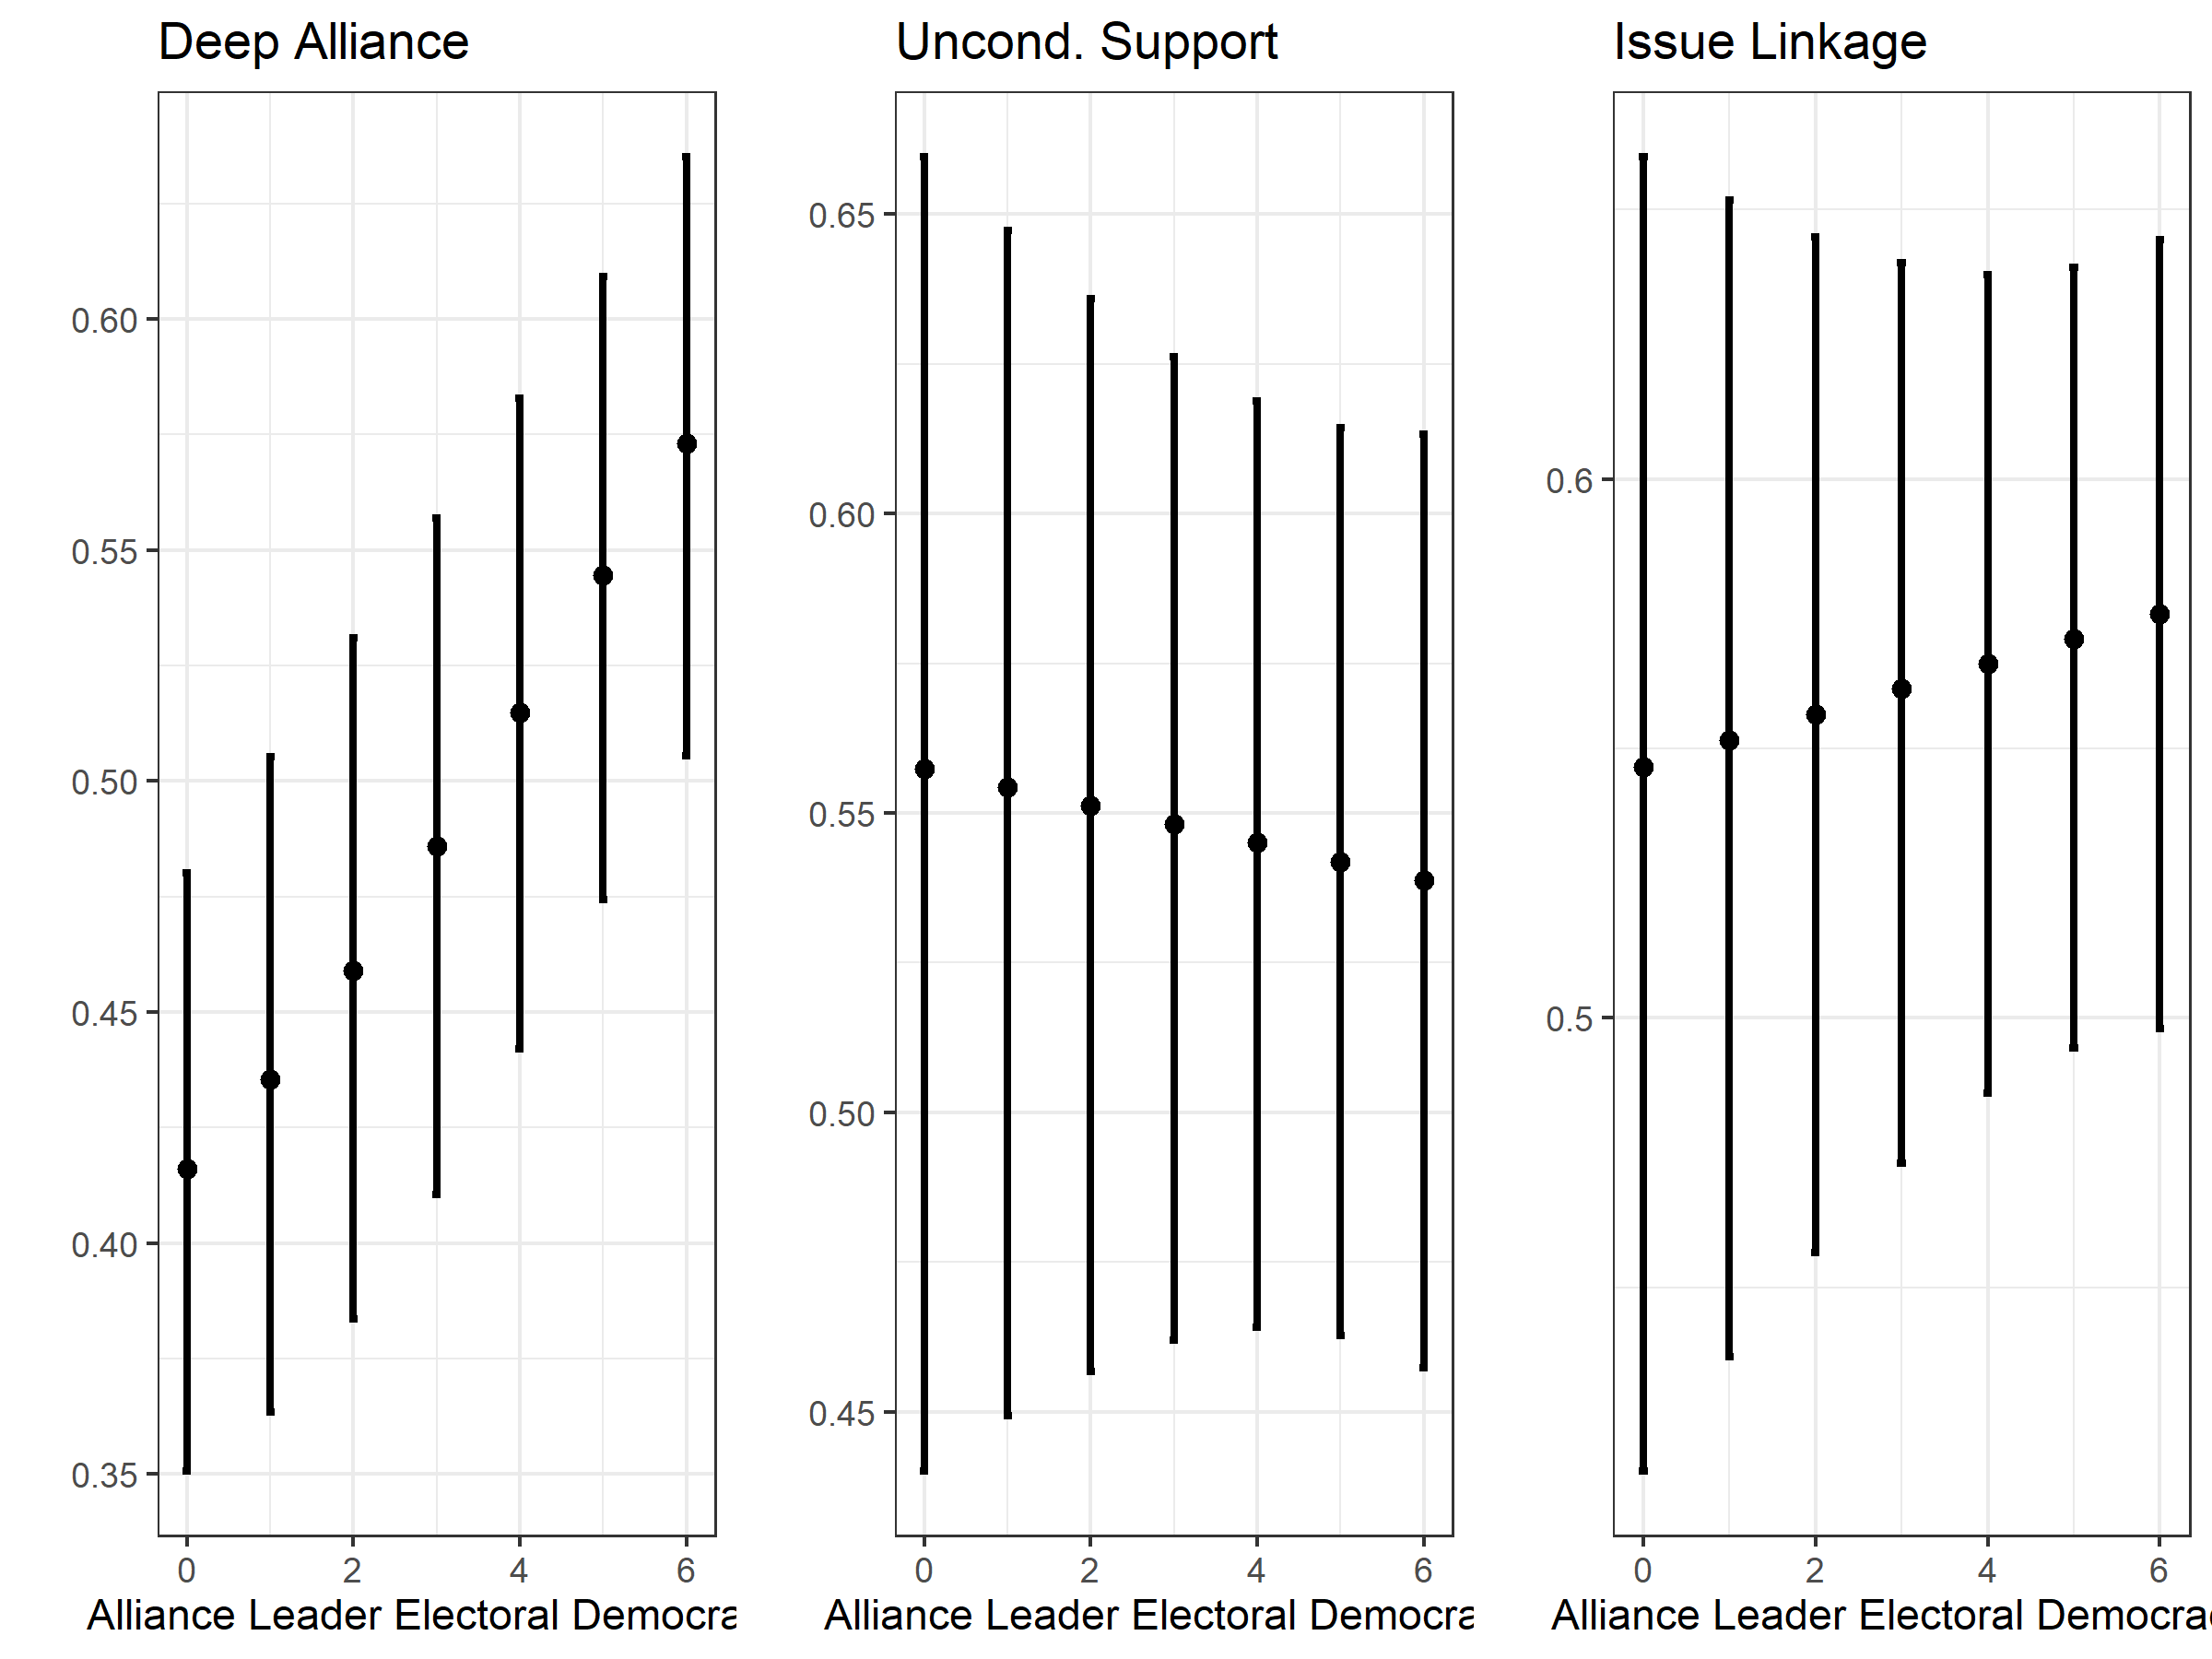
\includegraphics[width=.95\textwidth]{pred-trivar.png}  
\caption{Predicted probabilities an alliance includes treaty depth, unconditional military support or issue linkages for each value of alliance leader Polity scores. The three outcomes are dummy variables for a deep alliance, unconditional military support, and issue linkages. Predictions based on estimates from a trivariate GJRM with a normal copula.}
\label{fig:pred-trivar}
\end{figure}




\newpage

\singlespace
 
\bibliography{../../../MasterBibliography} 





\end{document}